\chapter{Metodologia}
\label{cap:Metodologia}

Dado que no Capítulo \ref{cap:Assistente} tratamos de apontar \textit{o que será desenvolvido}, neste capítulo buscamos expor \textit{os meios que usaremos} para alcançar o que nos propomos. Abordaremos, portanto, a definição de todos os elementos componentes da solução proposta, bem como os critérios utilizados nas tomadas de decisão quanto a recortes de dados de entrada e seu tratamento e preparação, modelos utilizados, critérios de avaliação e afins. Começamos, na Seção \ref{sec:Metodologia.1}, apontando a forma de preparação dos dados a serem consultados e usados como base para a geração final das respostas (sua seleção, tratamento, preparação e persistência no banco vetorial). A Seção \ref{sec:Metodologia.2} trata das decisões tomadas para realizar a melhor  configuração para o banco vetorial. As Seções \ref{sec:Metodologia.3} e \ref{sec:Metodologia.4} abordam, respectivamente, (1) a configuração do ambiente de execução do \ac{LLM} e (2) sua integração com os dados recuperados do banco vetorial -- efetivamente definindo a estrutura \ac{RAG}. A exposição da aplicação ao usuário, por meio de uma interface web simples é descrita na Seção \ref{sec:Metodologia.5}, ao passo que as medições dos resultados e avaliações são apresentadas na Seção \ref{sec:Metodologia.6}.

\section{Definição do Conjunto de Dados}
\label{sec:Metodologia.1}

Estabelecida a abordagem a ser utilizada para o desenvolvimento da ferramenta proposta, tornou-se necessário definir quais conjuntos de dados/documentos seriam incluídos no processo de desenho, implementação, testes e validação dos resultados. Dado que, conforme apresentado na Seção \ref{sec:DocAlern.1}, há, no contexto da \ac{Alern}, diferentes conjuntos de documentos com características diversas, tanto mais estáticos quanto extremamente dinâmicos, era necessário começar definindo que tipos de documentos e quais domínios dentre todos seriam significativos.

A escolha dos dados para desenvolvimento foi feita com o intuito de se alcançar dois objetivos específicos. O primeiro seria garantir que o objeto final dessa fase preliminar de desenvolvimento pudesse ser de uso relevante para a Casa Legislativa, tanto em termos de funcionalidade, mas também no sentido de abarcar um conjunto de informações que seja de interesse e relevância aos usuários do público interno ou externo à \ac{Alern}. Além deste, pretende-se assegurar que o domínio em que se enquadre o corpus escolhido coincida com as áreas de conhecimento e atuação dos integrantes do grupo de especialistas que se voluntariaram a avaliar a qualidade das respostas geradas. Com isso, seria potencializado o processo de testes e validação dos resultados da aplicação, tanto pelo volume de pessoas que poderão utilizar na fase de testes -- dado que informações escolhidas de forma estratégica atrairão mais usuários -- quanto pela qualidade do conhecimento dos avaliadores.

O recorte de documentos selecionados para compor o corpus textual sobre o qual esta proposta atuará foi feito sob sugestão e orientação de servidores atuantes nos setores de gestão de pessoas (CDHO - Coordenadoria de Desenvolvimento Humano e Organizacional) e setores envolvidos em diversas fases do processo legislativo -- em especial por serem a gestão de pessoas e o processo legislativo duas áreas da \ac{Alern} em que é comum o surgimento de dúvidas procedimentais, bem como a busca por informações que pautem ou desabonem uma ou outra medida a ser tomada ou ações dos servidores em geral. A coleção de documentos inclui a normatização e regimentação da atuação parlamentar, a regulação de direitos e deveres dos servidores (em especial no que se refere a benefícios/auxílios, cálculo de vencimentos, férias e bonificações), planos de cargos e carreiras, avaliação do servidor em estágio probatório de trabalho, assim como o regime jurídico dos servidores do Rio Grande do Norte (dos quais os servidores da \ac{Alern} são um subconjunto).

Os documentos selecionados têm suas características detalhadas nas Tabelas \ref{tab:descricao-documentos-1} e \ref{tab:descricao-documentos-2}. A Tabela \ref{tab:descricao-documentos-1} contém os quantitativos de \textit{tokens}, palavras e artigos em cada documento. A Tabela \ref{tab:descricao-documentos-2}, por sua vez, caracteriza a distribuição média de palavras e \textit{tokens} por artigo, em cada documento, bem como expõe a quantidade de artigos com mais de 300 palavras e com mais de 500 \textit{tokens} em cada documento -- sendo esse segundo dado algo relevante de se considerar, dado a limitação da quantidade de \textit{tokens} suportada por modelos específicos (ver início da Seção \ref{subsec:Metodologia.1.1} para mais detalhes).

Os documentos descritos nas Tabelas \ref{tab:descricao-documentos-1} e \ref{tab:descricao-documentos-2} -- identificados na primeira coluna de cada uma -- são
os seguintes:

\begin{enumerate}
    \item Lei Complementar Estadual Nº 122/1994
    \item Resolução Nº 031/2021 – Alern
    \item Resolução Nº 075/2024 – Alern
    \item Resolução Nº 078/2024 – Alern
    \item Resolução Nº 106/2018 – Alern
    \item Resolução Nº 2388/2019 – Alern
    \item Resolução Nº 077/2024 – Alern
    \item Resolução Nº 089/2017 – Alern
    \item Resolução Nº 618/2022 – Alern
    \item Resolução Nº 064/2022 – Alern
    \item Resolução Nº 133/2025 – Alern
    \item Manual de Processo Legislativo - Alern
\end{enumerate}

\begin{table}
    \caption{Quantitativos de Palavras/\textit{Tokens}/Artigos por Documento}
    \centering
    \begin{tabular}{ c c c c }
        \hline
        \textbf{Documento} & \textbf{palavras} & \textbf{\textit{tokens}} & \textbf{artigos} \\  
        \hline
        1 & 15.228 & 23.079 & 245 \\
        2 & 43.579 & 65.850 & 376 \\
        3 & 651 & 1.197 & 7 \\
        4 & 1.778 & 2.648 & 21 \\
        5 & 4.735 & 6.903 & 46 \\
        6 & 1.573 & 2.329 & 14 \\
        7 & 511 & 758 & 7 \\
        8 & 4.361 & 6.306 & 41 \\
        9 & 1.024 & 1.546 & 9 \\
        10 & 432 & 651 & 7 \\
        11 & 1.891 & 2.881 & 25 \\
        12 & 19.710 & 30.036 & ** \\
        \hline
    \end{tabular}
    
    \small \textbf{**Nota}: texto não articulado.
    
    Fonte: O autor (2025)
    \label{tab:descricao-documentos-1}
\end{table}

\begin{table}
    \caption{Quantitativos Palavras e \textit{Tokens} por Artigo em cada Documento}
    {
        \centering
        \begin{tabular}{ c c c c c }
            \hline
            \textbf{Documento} & \textbf{pals./art.} & \textbf{tokens/art.} & \textbf{arts. 300+ pals} & \textbf{arts. 500+ tokens} \\  
            \hline
            1 & 62,2 & 94,2 & 2 & 7 \\
            2 & 115,9 & 175,1 & 33 & 58 \\
            3 & 93,0 & 171,0 & 1 & 1 \\
            4 & 84,7 & 126,1 & 1 & 1 \\
            5 & 102,9 & 150,1 & 2 & 6 \\
            6 & 112,4 & 166,4 & 1 & 3 \\
            7 & 73,0 & 108,3 & 0 & 0 \\
            8 & 106,4 & 153,8 & 2 & 6 \\
            9 & 113,8 & 171,8 & 1 & 3 \\
            10 & 61,7 & 93,0 & 0 & 0 \\
            11 & 75,64 & 114,76 & 0 & 0 \\
            12 & ** & ** & ** & ** \\
            \hline
        \end{tabular}
    }

    \small \textbf{**Nota}: texto não articulado.\\
    \small \textbf{pals./art.}: Média do número de palavras por artigo \\
    \small \textbf{tokens/art.}: Média do número de \textit{tokens} por artigo \\
    \small \textbf{arts. 300+ pals}: Número de artigos com mais de 300 palavras \\
    \small \textbf{arts. 500+ tokens}: Número de artigos com mais de 500 \textit{tokens} \\
    
    {\centering
        Fonte: O autor (2025)\par
    }
    \label{tab:descricao-documentos-2}
\end{table}

Ao se analisar os elementos do conjunto de documentos selecionados, é possível perceber que há certo grau de homogeneidade entre os documentos em alguns quesitos. Alguns exemplos de proximidade entre esses componentes são a interrelação entre as temáticas, as suas estruturas semelhantes entre si, seguindo a divisão padrão de textos normativos -- com capítulos, seções, artigos, parágrafos, alíneas, etc. --, o tom do vocabulário e o estilo da escrita característicos de texto legislativo, entre outros. Essa homogeneidade, em especial no que se refere à estrutura, facilita sua manipulação, sua eventual fragmentação e seu processamento, em preparação para sua inclusão no fluxo de atividades do sistema.

Não obstante, também é facilmente perceptível que os exemplares da lista de documentos possuem características distintas entre si: há variação considerável no comprimento dos documentos como um todo, alguns são apenas leis que alteram a redação de outra peça existente no conjunto sem oferecer outros conteúdos, entre outras características que os diferenciam entre si. Também é relevante essa disparidade, visto que, mesmo dentro de um contexto de documentos semi-estruturados, há diversidade suficiente para que seu tratamento seja adequado e aplicável a textos puramente não estruturados.

Uma característica peculiar do conjunto de dados utilizado é a possibilidade de documentos normativos diferentes estabelecerem como fatos informações conflitantes e se contradizerem. Há duas situações, que conseguimos prever, nas quais é possível que haja choque de informações: atualização da regulação e especificidades hierárquicas.

A primeira se dá pelo motivo de que, pela própria dinâmica da atividade legislativa, determinadas leis/normas são atualizadas, modificadas ou criadas com o tempo; de forma que algo que é estabelecido como fato hoje pode ser impactado por um novo ato normativo, por alteração do texto da lei, por sua revogação e afins. De forma a mitigar essa problemática, é necessária a manutenção dos documentos e suas representações vetoriais, garantindo que sua versão mais atualizada (preferencialmente a versão compilada de seu texto) seja a disponibilizada pelo banco vetorial.

A segunda se dá quando uma peça normativa de abrangência maior prevê algo, enquanto um ato normativo de alcance específico preveem, paradoxalmente, coisas distintas. Um caso específico, para fins de demonstração, é o fato de o Regime Jurídico dos servidores públicos civis do Estado do Rio Grande do Norte determina que:

\begin{citacao}
    A gratificação natalina, devida a ocupante de cargo efetivo ou em comissão, corresponde a 1/12 (um doze avos) da remuneração a que fizer jus no mês de dezembro, por mês de exercício no respectivo ano \cite{RegimeJuridico:RN}.
\end{citacao}


Assim, enquanto no âmbito mais amplo do Estado do RN a gratificação natalina é calculada unicamente em função da remuneração base do servidor, a Resolução Nº 77, de 10 de julho de 2024 \cite{RegimentoInterno:ALRN}, que trata da base de cálculo do terço de férias e da gratificação natalina (13º salário) especificamente dos servidores da \ac{Alern} prevê que:
\begin{citacao}
    Fica determinado que os valores percebidos a título de auxílio-alimentação e auxílio de assistência à saúde, por se tratarem de vantagens pecuniárias que compõem a remuneração do servidor, serão incluídos na base de cálculo do terço constitucional de férias e da gratificação natalina (13º salário) dos servidores e, naquilo que couber, dos membros da Assembleia Legislativa do Estado do Rio Grande do Norte.
\end{citacao}

Como ambos os documentos estão disponíveis no banco vetorial, uma busca por ``Os valores recebidos como auxílio-alimentação compõem a base de cálculo para a gratificação natalina?'' pode resultar no retorno de ambos os fragmentos, provendo ao \ac{LLM} informações conflitantes, visto que não foi fornecido um contexto na pergunta. Embora seja possível uma abordagem mais efetiva para a resolução deste problema (como uma organização hierárquica -- em termos de abrangência -- dos documentos), no escopo deste estudo, limitamo-nos a informar ao \ac{LLM}, junto com o texto do fragmento, o seu título e autor, que por si só já delimitam o âmbito em que a peça normativa se aplica.

\subsection{Tratamento dos Dados Selecionados}
\label{subsec:Metodologia.1.1}

Feita a coleta dos arquivos com os textos dos documentos elencados para a composição do conjunto a ser utilizado, foi necessário definir como o texto seria tratado. Os aspectos de particionamento dos documentos e da manutenção do contexto do conteúdo são abordados nas Seções \ref{subsubsec:Metodologia.1.1.1} e \ref{subsubsec:Metodologia.1.1.2}, respectivamente.

\subsubsection{Fragmentação do Conteúdo}
\label{subsubsec:Metodologia.1.1.1}

Um dos aspectos que deve ser levado em consideração é a garantia de que o tamanho de seu conteúdo seja adequado às limitações das ferramentas de geração de representação vetorial do texto. Ignorar essas características de cada modelo pode levar à perda de informação quando da geração dos \textit{embeddings} dos documentos, dado que os modelos truncam parte do conteúdo sobre o qual operarão, nos casos em que o número máximo de \textit{tokens} que conseguem processar é extrapolado. A divisão ou particionamento do conteúdo textual dos documentos é a parte central desse processo.

Considerando que diversos modelos selecionados para avaliação na inclusão das funções de geração de \textit{embeddings} neste trabalho (ver Tabela \ref{tab:num-maximo-tokens} na Seção \ref{subsubsec:Metodologia.2.1.6}) têm uma limitação no número de \textit{tokens} de entrada para geração da representação em vetores (em geral 512 \textit{tokens}), visto que se baseiam na arquitetura \textit{Transformer}, \cite{Instructor:3}, a escolha feita foi pela fragmentação de cada um dos documentos em porções de texto com um número máximo de 300 palavras. Com isso, cada fragmento de um documento seria tratado pelo Chroma DB como um documento por si só, ficando sua relação de pertencimento registrada nos metadados, para casos de eventuais  buscas pelo documento como um todo. Dessa forma, ao serem \textit{tokenizados} os fragmentos dos documentos no conjunto, as representações vetoriais resultantes ficam dimensionadas de forma a respeitar a limitação de tamanho da entrada recebida pelo modelo utilizado, eliminando a necessidade de supressão de informações por truncamento dos \textit{tokens} excedentes.

A fragmentação do volume do texto de fato é desejável e otimiza o processo de recuperação de documentos (fragmentos menores permitem maior granularidade no cálculo da semelhança semântica com o \textit{input} do usuário), além de reduzir o tamanho geral do \textit{prompt} a ser fornecido ao \ac{LLM} para geração do conteúdo sintético a responder a pergunta feita, visto que este incluirá o conteúdo dos fragmentos recuperados. Todavia, a divisão do conteúdo considerando meramente o tamanho de cada fragmento pode implicar em dispersão de contexto, colocando uma parte de uma ideia em um fragmento, isolando-a de sua parte complementar alocada em outro, de forma que a ideia completa se perde no instante da recuperação de documentos, podendo não ser identificada pela busca semântica de similaridade.

\subsubsection{Manutenção do Contexto}
\label{subsubsec:Metodologia.1.1.2}

Considerando o exposto na Seção anterior, é igualmente crucial mitigar a fragmentação e dispersão do contexto dos dados, evitando que informações correlacionadas -- e contíguas, no texto original -- se encontrem espalhadas ao longo de diversos fragmentos ao final do processo de divisão dos documentos em pedaços menores. Para isso é importante compreender que o sentido, o significado e a semântica comunicados residem não somente o conteúdo textual, nas palavras expressas do texto, senão também no que se infere a partir do que os precedeu, seja a nível textual ou estrutural.

Assim, realizar a divisão do documento garantindo que os pontos de quebra aconteçam entre uma frase e outra -- depois de um ponto final/interrogação/exclamação -- garante que ideias não sejam quebradas no nível da frase, reduzindo em parte a fratura de contexto que se realiza considerando meramente o número de palavras/\textit{tokens} do fragmento final. Igualmente, a garantia de que a quebra acontece em um ponto que divide duas unidades com um grau maior de completude de uma ideia avança na direção de se obter fragmentos semanticamente autocontidos, com menor dependência de conteúdo conseguinte ou, ainda mais, precedente. Com efeito, o contexto precedente possui impacto maior sobre a completude de uma partição do documento do que aquele que a sucede.

Além da informação textual que antecede certo excerto, muito sentido é codificado na estrutura do documento em si -- em especial nos casos de documentos formalmente estruturados e/ou organizados de forma hierárquica. 

Considere, por exemplo, o texto seguinte organizado hierarquicamente:

\fbox{%
  \parbox{0.75\linewidth}{%
    \raggedright \sffamily
    \textbf{Preparação do Ambiente} \\
    Como forma de facilitar o processo de adaptação, mudanças e atualização, optamos por adotar um cliente LLM chamado Ollama. Mais informações a respeito em \href{https://ollama.com/}{https://ollama.com/}.

    \vspace{6pt}
    \textbf{Linux} \\

    \textbf{Como instalar o Ollama}
    \begin{itemize}
      \item No terminal, baixe e execute o script de instalação:
      \item \texttt{curl -fsSL https://ollama.com/install.sh | sh}
    \end{itemize}

    \textbf{Como definir as variáveis de ambiente}
    \begin{itemize}
      \item \texttt{export OLLAMA\_MAX\_LOADED\_MODELS=5}
      \item \texttt{export OLLAMA\_DEBUG='true'}
    \end{itemize}

    \vspace{6pt}
    \textbf{Windows} \\

    \textbf{Como instalar o Ollama}
    \begin{itemize}
      \item Acesse a página de download do Ollama no link \href{https://ollama.com/download/windows}{https://ollama.com/download/windows} e faça o download do instalador.
      \item Execute o instalador e siga as instruções em tela.
    \end{itemize}

    \textbf{Como definir as variáveis de ambiente}

    \textbf{Powershell}
    \begin{itemize}
      \item \texttt{\$env:OLLAMA\_MAX\_LOADED\_MODELS=5; \$env:OLLAMA\_DEBUG=`true'}
    \end{itemize}

    \textbf{Prompt}
    \begin{itemize}
      \item \texttt{set OLLAMA\_MAX\_LOADED\_MODELS=5}
      \item \texttt{set OLLAMA\_DEBUG=`true'}
    \end{itemize}
  }
}

Ignorando o comprimento diminuto de cada uma das seções -- tomando-as como mais longas -- vemos que temos duas seções com informações diferentes de como instalar o Ollama. O que as torna coerentes não é o conteúdo de cada uma, mas o ponto da hierarquia da estrutura textual em que ambas se localizam. Destarte, é necessário ``injetar'' no texto dos fragmentos que compõem ambas essas seções informações sobre sua posição na estrutura hierárquica do documento.

O mesmo princípio se aplica a documentos articulados, como peças legislativas, em que as alíneas e parágrafos, por exemplo, só têm coerência semântica quando vinculados com as informações antecedentes, dentro do mesmo artigo.

\subsubsection{Documentos Articulados}
\label{subsubsec:Metodologia.1.1.3}

Diante do exposto, como uma abordagem para minimizar essa dispersão contextual, o processo de segmentação dos documentos se utilizou da estrutura intrínseca de cada um deles (divisão em artigos, parágrafos, alíneas e afins, nos casos de documentos articulados), de forma que os fragmentos ficaram orientados à divisão por artigo, dado que cada artigo é uma unidade autocontida, semanticamente coerente, sendo, no grosso dos exemplos, independente dos outros artigos, salvo quando de citação e referência. Mais claramente, cada documento foi segmentado de tal sorte que cada artigo compõe um fragmento. Apesar disso, conforme se vê na Tabela \ref{tab:descricao-documentos-2}, ainda há, no corpus selecionado, 43 artigos cujo teor textual ultrapassa o número de 300 palavras (via de regra por conter um grande número de parágrafos, incisos e alíneas), incorrendo no mesmo problema que ora é abordado, exceto que em um número muito menor de ocorrências, dada a raridade de artigos longos no conjunto de dados em questão.

Como uma forma de evitar essa situação, a abordagem adotada foi, nos casos de artigos mais extensos, secionar adicionalmente o artigo, em suas partes menores (caput, parágrafos, incisos e alíneas) e agrupá-las de forma que cada um desses agrupamentos consista de uma combinação do caput e parágrafos/incisos/alíneas cujo comprimento total não ultrapasse o limite escolhido de 300 palavras, conforme a Figura \ref{fig:fragmentacao-artigos}. Assim, embora essa fragmentação automatizada -- independente de divisão feita sob análise caso a caso -- não resolva o problema em sua completude, ao se garantir que cada um desses segmentos mantenha o contexto geral do artigo, condensado no caput, mitiga-se uma fragmentação extrema da ideia geral do artigo, obtendo-se uma coesão maior do que haveria no caso da divisão com base somente no número de palavras.

\begin{figure}[H]
    \centering
    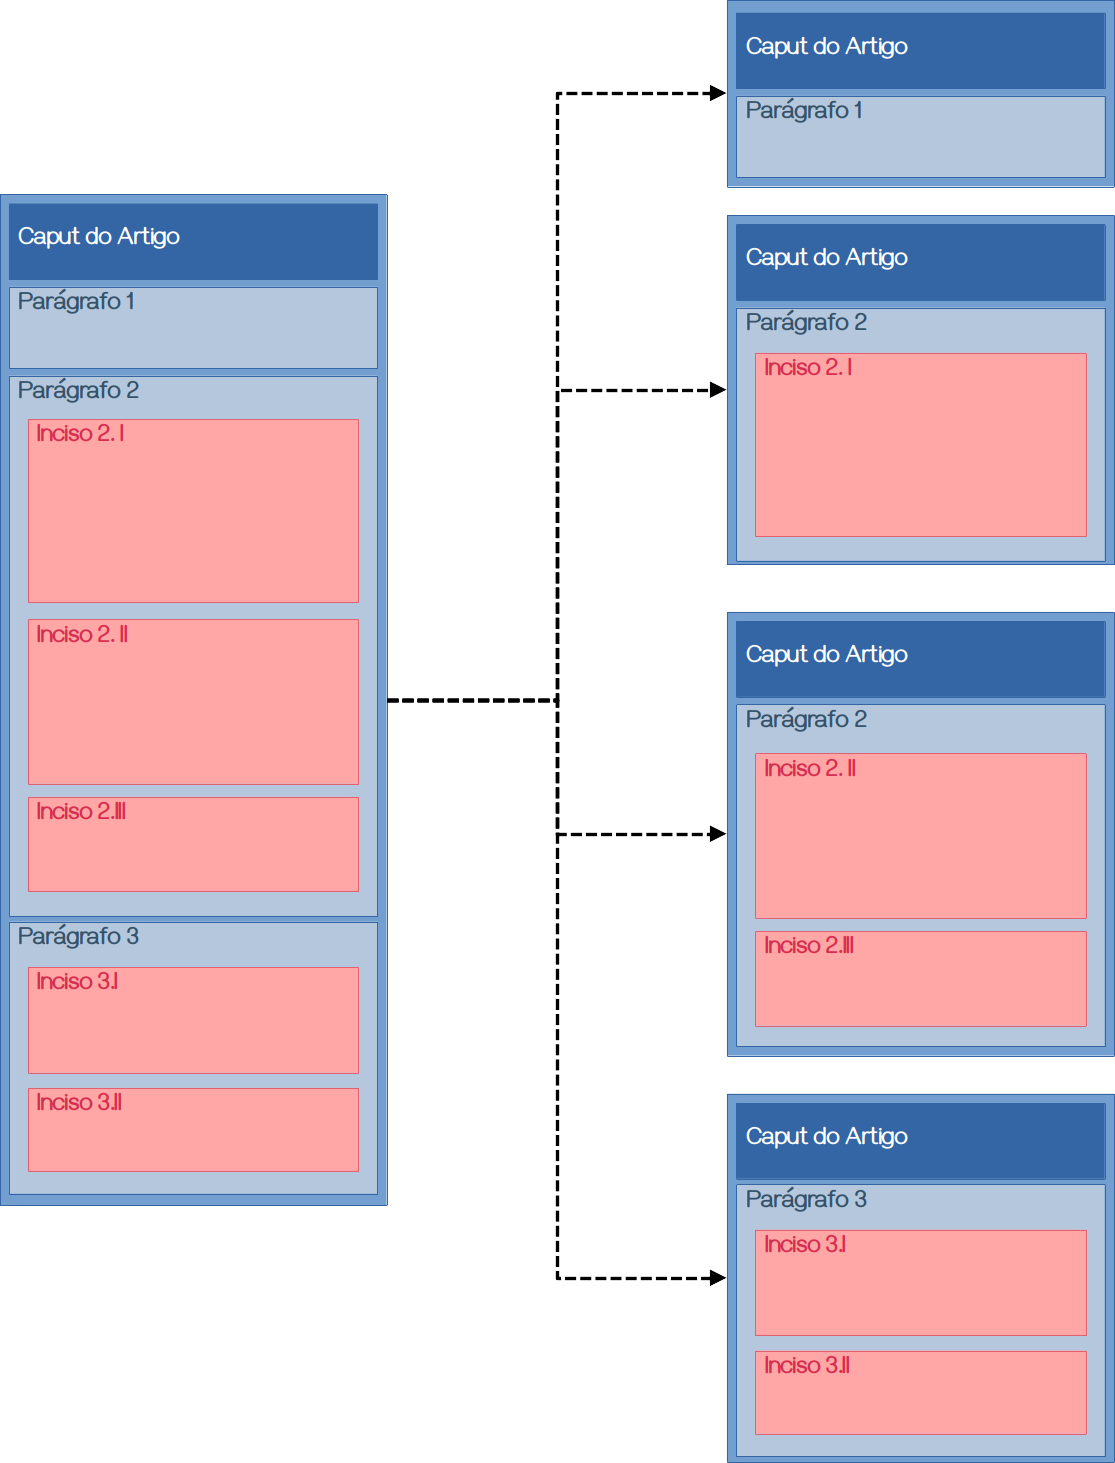
\includegraphics[width=0.5\linewidth]{Imagens/fragmentacao-artigos.png}
    \caption{Estratégia de Fragmentação de Artigos Extensos}
    Fonte: autoria própria
    \label{fig:fragmentacao-artigos}
\end{figure}

O resultado final do quantitativo de fragmentos por documento articulado está descrito na Tabela \ref{tab:descricao-fragmentos-1}.

\begin{table}[H]
    \caption{Quantitativos de artigos e Fragmentos por Documento}
    {
        \centering
        \begin{tabular}{ l c c c }
            \hline
            \textbf{Documento} & \textbf{Artigos} & \textbf{300+} & \textbf{Fragmentos} \\  
            \hline
            1. Lei Complementar Estadual Nº 122/1994 & 245 & 2 & 248 \\
            2. Resolução Nº 031/2021 – Alern & 376 & 33 & 420 \\
            3. Resolução Nº 075/2024 – Alern & 7 & 1 & 8 \\
            4. Resolução Nº 078/2024 – Alern & 21 & 1 & 22 \\
            5. Resolução Nº 106/2018 – Alern & 46 & 2 & 48 \\
            6. Resolução Nº 2388/2019 – Alern & 14 & 1 & 15 \\
            7. Resolução Nº 077/2024 – Alern & 7 & 0 & 7 \\
            8. Resolução Nº 089/2017 – Alern & 41 & 2 & 44 \\
            9. Resolução Nº 618/2022 – Alern & 9 & 1 & 10 \\
            10. Resolução Nº 064/2022 – Alern & 7 & 0 & 7 \\
            11. Resolução Nº 133/2025 - Alern & 25 & 0 & 25 \\
            12. Manual de Processo Legislativo & ** & ** & 244 \\
            \hline
        \end{tabular}
    }

    \small \textbf{**Nota}: O Manual de Processo Legislativo não é articulado (ver Seção \ref{subsubsec:Metodologia.1.1.4}) \\
    \small \textbf{300+}: Número de artigos com mais de 300 palavras \\
    
    {\centering
        Fonte: O autor (2025)\par
    }
    \label{tab:descricao-fragmentos-1}
\end{table}


\subsubsection{Documento Hierárquico}
\label{subsubsec:Metodologia.1.1.4}

Para realizar o particionamento do documento não articulado (O Manual de Processo mencionado e descrito na Seção \ref{sec:Metodologia.1}, mais especificamente nas Tabelas \ref{tab:descricao-documentos-1} e \ref{tab:descricao-documentos-2}), nos apoiamos em sua estrutura hierárquica. Definimos o limite de tamanho do fragmento tal qual no caso de documentos articulados (Seção \ref{subsubsec:Metodologia.1.1.1}) e aplicamos a ideia de autocontenção de conteúdo nos fragmentos, de forma que cada um deles tenha o máximo de autonomia semântica possível (Seção \ref{subsubsec:Metodologia.1.1.2}).

Dado que o documento não é articulado, tomamos como unidade semanticamente atômica o parágrafo. E como forma de injetar informação sobre o contexto hierárquico a que o fragmento pertence, lançamos mão dos cabeçalhos de cada seção/subseção no nível superior ao do fragmento. A Figura \ref{fig:fragmentacao-hierarquico} mostra a estratégia de particionamento de arquivos hierárquico.

\begin{figure}[H]
    \centering
    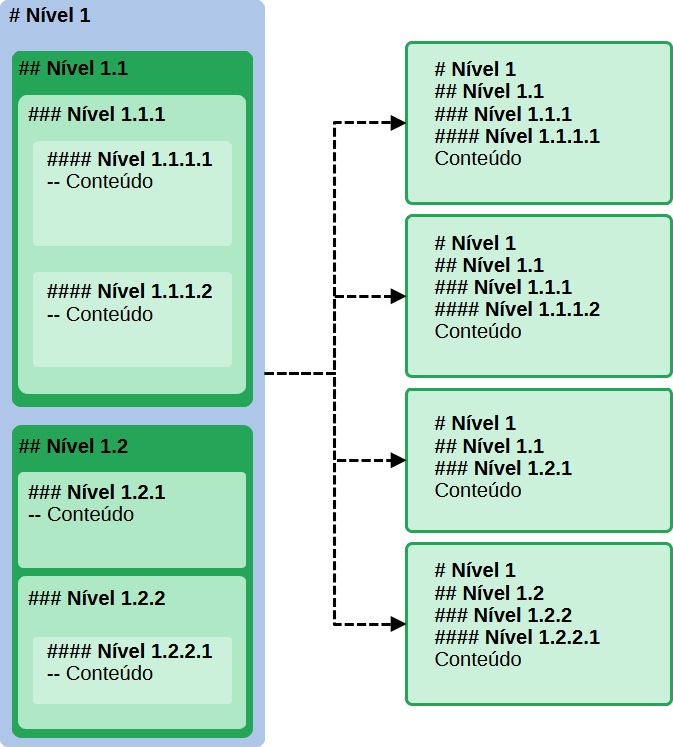
\includegraphics[width=0.5\linewidth]{Imagens/fragmentacao-hierarquico.png}
    \caption{Estratégia de Fragmentação de Arquivos Hierárquicos}
    Fonte: autoria própria
    \label{fig:fragmentacao-hierarquico}
\end{figure}

Assim, se aplicássemos essa abordagem sobre o exemplo de texto hierárquico que usamos anteriormente, o fragmento que contém a segunda seção chamada ``Como instalar o Ollama'' ficaria com o seguinte conteúdo:

    \begin{quote}
    {
        \begin{minipage}{\dimexpr\linewidth-2em}
        \setlength{\rightskip}{0.7em}
        \footnotesize
        \ttfamily
        \raggedright
        \sloppy
        Preparação do Ambiente
        
        Windows
        
        Como instalar o Ollama
        
        - Acesse a página de download do Ollama no link\\
        https://ollama.com/download/windows\\
        e faça o download do instalador.
        - Execute o instalador e siga as instruções em tela
        \end{minipage}
    }
    \end{quote}

Dessa forma, mantivemos indicadores explícitos que sinalizam a posição do fragmento dentro da estrutura geral do documento incorporados ao conteúdo textual da seção, aplicando algum grau de redução da dispersão de informação e perda de dados contextuais.

\section{Definindo o Banco Vetorial}
\label{sec:Metodologia.2}
Havendo sido separados os dados de interesse para a aplicação, era necessário organizar o banco vetorial (Seção \ref{sec:Assistente.1}) em que estes seriam representados, armazenados e disponibilizados às consultas. Dado que a opção feita foi pelo Chroma DB (Seção \ref{subsec:Assistente.1.1}), o qual se trata de um banco vetorial que, com fins de otimização de desempenho, opera ``em memória'', não carecendo de instalação no sentido estrito da palavra -- diferindo dos \ac{SGBD}s tradicionais --, bastando somente instalar a biblioteca Python disponibilizada pela Chroma, visto que utilizaremos essa linguagem de programação para integrar as partes/módulos do assistente (ver Seção \ref{sec:Metodologia.4}). Agora, portanto, tratamos dos aspectos de configuração do banco Chroma DB para, posteriormente, receber os dados que serão servidos nas buscas dos usuários.

\subsection{Escolhendo o modelo de Embeddings}
\label{subsec:Metodologia.2.1}
A Seção \ref{subsec:Assistente.1.2} apresentou a possibilidade de fornecer ao Chroma DB uma função de geração de \textit{embeddings} personalizada, permitindo escolher qual modelo de representação vetorial ser utilizado. Tratamos, nesse ponto do estudo, de definir, dentre um conjunto de modelos candidatos, qual teria o melhor desempenho em termos de recuperação de conteúdo relevante em relação à consulta feita. A seleção de modelos feita incluiu os seguintes modelos: (1) \textit{instructor-xl}, (2) \textit{text-embedding-ada-002} (ao qual nos referiremos como \textit{ada-002}, (3) \textit{text-embedding-3-large} (que nominaremos como \textit{3-large}), (4) \textit{GTE}, (5) \textit{BGE-m3}, (6) \textit{Llama3.1}, (7) \textit{DeepSeek-r1} e (8) \textit{BERT-QA}. Apresentamos, a seguir, cada um deles.

\subsubsection{instructor-xl}
\label{subsubsec:Metodologia.2.1.1}

Dentre os modelos avaliados, o que mais chamou atenção foi o \textit{instructor-xl} dada a sua proposta de flexibilidade. Trata-se de um modelo desenvolvido pela equipe de pesquisa de Processamento de Linguagem Natural (NLP) da Universidade de Hong Kong, incluindo a participação de pesquisadores de outras instituições, como \textit{University of Washington}, Meta AI e \textit{Allen Institute for AI}, publicado em 2023 \cite{Instructor:1}. O modelo selecionado pertence à série de modelos INSTRUCTOR, que são projetados para gerar \textit{embeddings} de texto de alta qualidade e se baseiam na arquitetura \textit{Transformer}, assim como modelos de estado da arte, como \ac{BERT} e \ac{GPT}.

No trabalho de  \citeonline{Instructor:2}, os seus publicadores o definem como \textit{``One Embedder [for] Any Task''} (Um Gerador de \textit{Embeddings} para Qualquer Tarefa) e como

\begin{citacao}
    \textit{an instruction-finetuned text embedding model that can generate text embeddings tailored to any task (e.g., classification, retrieval, clustering, text evaluation, etc.) and domains (e.g., science, finance, etc.) by simply providing the task instruction, without any finetuning.} \footnote{Um modelo de geração de \textit{embeddings} textuais com \textit{fine-tuning} feito a partir de uma instrução, capaz de gerar \textit{embeddings} de texto otimizados para qualquer tarefa (tais como, classificação, recuperação, agrupamento, avaliação de texto, etc.) e quaisquer domínios (quais sejam ciência, finanças, etc.) simplesmente fornecendo a instrução da tarefa, sem necessidade de \textit{fine-tuning} tradicional. (Tradução nossa)}
\end{citacao}

Os INSTRUCTORs são, portanto, modelos de criação de \textit{embeddings} textuais de forma adaptativa. Em vez de gerar \textit{embeddings} baseando-se unicamente nos parâmetros alcançados em seu treinamento, ele lança mão de instruções em linguagem natural fornecidas no momento de sua execução, as quais devem descrever as tarefas em que os \textit{embeddings} serão utilizados. Ao utilizar as instruções como elementos ``direcionadores'' do processo de geração de \textit{embeddings}, pretende-se que o resultado final seja otimizado para as tarefas definidas, fazendo as vezes de um ``ajuste fino''. Essa abordagem demonstra, segundo os seus desenvolvedores, bom desempenho em não somente ``compreender'' texto em um sentido mais aberto e genérico, sendo capaz, também, de interpretá-lo com uma visão direcionada a aplicações e casos de uso particulares.

Desta forma, as representações vetoriais geradas são otimizadas para tarefas específicas (como classificação, recuperação de informações, agrupamento, avaliação semântica, entre outras) e/ou domínios diferentes, sem a necessidade de refinamento do modelo nos moldes tradicionais de \textit{finetuning}, tornando-o adaptável e mais relevante para diversas aplicações.
A versão do modelo que escolhemos testar para possível uso no Assistente de Busca, especificamente, é a \textit{instructor-xl}, sendo a variante dentre a família de modelos INSTRUCTOR com maior tamanho, otimizada para desempenho e equilíbrio entre precisão e eficiência em aplicações de \ac{PLN}, podendo ser utilizada por meio do \textit{framework} \textit{sentence-transformer}, disponibilizado pelo \textit{HuggingFace}, como \textit{hkunlp/instructor-xl}.

\subsubsection{text-embedding-ada-002}
\label{subsubsec:Metodologia.2.1.2}

Outro modelo selecionado por ser promissor foi o \textit{text-embedding-ada-002}, desenvolvido e oferecido como um serviço pela OpenAi desde o final do ano de 2022. A página de apresentação do modelo o descreve como a unificação de cinco modelos anteriores (\textit{text-similarity}, \textit{text-search-query}, \textit{text-search-doc}, \textit{code-search-text} and \textit{code-search-code}) em um único modelo aprimorado, alcançando melhores resultados em busca textual, similaridade de frases e \textit{benchmarking} de busca em código \cite{ADA:1}.

Um dos pontos positivos apontados na página é o fato de utilizar uma forma compacta de representação em \textit{embeddings} (apenas 1.536 dimensões), apresentando melhor custo-benefício para utilização em bancos vetoriais, a despeito do suporte a um contexto maior. A isso adiciona-se o fato de ser menos computacionalmente custoso de se utilizar, dado que o processamento é delegado à API da OpenAI, enviando o texto a ser processado, via requisição HTTP e recebendo os \textit{embeddings} como resposta.

Como ponto negativo há o custo atrelado a cada requisição feita à API, tanto para gerar os \textit{embeddings} dos documentos quanto, posteriormente, para gerar os \textit{embeddings} de cada consulta feita ao banco de vetores, enquanto houver utilização da aplicação.

Embora não seja o modelo mais recente, dado que outros modelos mais eficientes e comparativamente baratos hajam sido lançados pela OpenAi, o posicionamento da empresa é de que o \textit{ada-002} não está sendo declarado como obsoleto (\textit{deprecated}) de forma que, embora recomendem o \textit{text-embedding-3-large}, seu modelo mais novo (ver a Seção \ref{subsubsec:Metodologia.2.1.3}), os clientes podem continuar usando o \textit{ada-002}.\footnote{``We are not deprecating text-embedding-ada-002, so while we recommend the newer model, customers are welcome to continue using the previous generation model'' \cite{3_large:1}.}

\subsubsection{text-embedding-3-large}
\label{subsubsec:Metodologia.2.1.3}

Lançado em janeiro de 2024, o modelo \textit{text-embedding-3-large}, juntamente com o \textit{text-embedding-3-small}, representa uma nova geração de modelos de vetorização textual desenvolvidos pela OpenAI, caracterizando-se por sua maior capacidade e desempenho superior em tarefas de representação semântica. Este modelo é capaz de gerar \textit{embeddings} com até 3.072 dimensões, o que possibilita uma codificação mais rica e detalhada de textos em espaços vetoriais de alta dimensionalidade.

O modelo \textit{text-embedding-3-large} apresenta desempenho substancialmente superior ao \textit{text-embedding-ada-002}, com destaque para os ganhos observados nos \textit{benchmarks} MIRACL (de 31,4\% para 54,9\%) e MTEB (de 61,0\% para 64,6\%), indicando avanços consistentes na qualidade dos \textit{embeddings} em tarefas de recuperação de informações, similaridade semântica, classificação e ranqueamento.

A adoção do \textit{text-embedding-3-large} é, portanto, recomendada para aplicações que exigem representações vetoriais de alta fidelidade, particularmente em contextos multilíngues e domínios que demandam precisão semântica elevada.


\subsubsection{GTE}
\label{subsubsec:Metodologia.2.1.4}
Desenvolvida pela \textit{Aliyun} ou \textit{Alibaba Cloud}, uma das subsidiárias do conglomerado chinês Alibaba Group voltada para o mercado de computação em nuvem, a série de modelos \textit{GTE-Multilingual} (\textit{mGTE}) -- uma reformulação do \textit{General Text Embedding} (\textit{GTE}) -- foi apresentada em novembro de 2024. A empresa aponta que o conjunto de modelos

\begin{citacao}
    \textit{offers high performance, long-context handling, multilingual support, and elastic embedding, significantly improving retrieval and ranking efficiency (...) [being, therefore,] suitable for a wide range of advanced \ac{RAG} applications} \cite{GTE:1}.
    \footnote{oferece um alto desempenho, tratamento de contextos longos, suporte multi-idiomas e \textit{embeddings} com tamanho ajustável, aprimorando significativamente a eficiência na recuperação e re-rankeamento/reclassificação, (...) [sendo, portanto,] adequadas ao uso em uma ampla gama de aplicações avançadas de \ac{RAG}. (Tradução nossa)}
\end{citacao}

O conjunto inclui ``modelos base, modelos de \textit{embeddings} e de \textit{ranking}'' \cite{GTE:1}, com resultados promissores particularmente para tarefas de recuperação de documentos, sendo amplamente utilizados como modelos de referência por organizações como a PostgresML \cite{GTE:2}. Dado que em sua própria documentação e material de divulgação dos modelos o \textit{mGTE} é referido simplesmente como \textit{GTE}, adotaremos aqui a mesma nomenclatura.

Assim como com o \textit{instructor-xl}, também é possível utilizar o \textit{GTE} com o \textit{sentence-transformer}, como \textit{Alibaba-NLP/gte-multilingual-base}.

\subsubsection{BGE-m3}
\label{subsubsec:Metodologia.2.1.5}
O \textit{BGE-m3} é um modelo desenvolvido por pesquisadores da \textit{Beijing Academy of Artificial Intelligence} -- BAAI (uma organização de pesquisa em inteligência artificial, sem fins lucrativos, também conhecida como \textit{Zhiyuan Institute}) e da \textit{University of Science and Technology of China}. Os autores o apontam como um modelo distinto dos demais em termos de versatilidade, considerando três frentes distintas: multilinguística, multifuncionalidade e multigranularidade.

Apontam \citeonline{BGE:1} que o \textit{M3-Embedding} foi capaz de abstrair um ``espaço semântico comum'' a todas as línguas sobre as quais foi feito o processo de treinamento, permitindo-lhe demonstrar competência na recuperação de conteúdo semanticamente semelhante com suporte a mais de 100 idiomas. Adicionalmente, dado que sua representação interna é feita sobre essa camada semântica abstrata compartilhada, é possível realizar recuperação de conteúdo interlinguístico.

No que concerne a multifuncionalidade e multigranularidade,

\begin{citacao}
    \textit{[M3-Embedding] is able to generate versatile embeddings to support different retrieval functionalities, not just dense retrieval, but also sparse retrieval and multivector retrieval. Finally, M3-Embedding is learned to process different input granularities, spanning from short inputs like sentences and passages, to long documents of up to 8,192 input tokens.} \cite{BGE:1}
    \footnote{[O \textit{M3-Embedding}] é capaz de gerar \textit{embeddings} versáteis que viabilizam múltiplas funcionalidades de recuperação da informação, abrangendo não apenas a recuperação densa, mas também a recuperação esparsa e a recuperação por multivetores. Por fim, o \textit{M3-Embedding} é treinado para lidar com diferentes granularidades de entrada, variando desde entradas curtas, como frases e excertos, até documentos extensos, com até 8.192 \textit{tokens} de entrada. (Tradução nossa)}
\end{citacao}

O modelo também é utilizável a partir do \textit{framework} do HuggingFace como \textit{BAAI/BGE-m3}, tornando simples a sua utilização no projeto.

\subsubsection{Outros Modelos}
\label{subsubsec:Metodologia.2.1.6}
Durante o processo de escolha dos modelos a serem usados na função para gerar os \textit{embeddings} a serem utilizados no banco vetorial, apercebemo-nos de que a ferramenta Ollama (abordada na Seção \ref{subsec:Assistente.2.3}, de cujos detalhes de implementação trata a Seção \ref{sec:Metodologia.3}) possui a funcionalidade de utilização de modelos diversos para geração de \textit{embeddings}. Dado que já incluíramos \ac{LLM}s na ferramenta, decidimos incluí-los no conjunto de modelos a serem testados para geração de representações vetoriais na aplicação.

Ademais, quando da análise exploratória de abordagens do problema objeto deste estudo, encontramos modelos treinados especificamente para utilização em aplicações de perguntas e respostas (\textit{Q\&A Systems}), de forma que, na fase de realização de testes de desempenho dos modelos, já estava um deles disponível nos dispositivos de execução do projeto. Sendo esse modelo específico capacitado à geração de \textit{embeddings}, optamos por também incluí-lo no rol de modelos a serem avaliados.

É importante notar, todavia, que os \ac{LLM}s e o modelo com ajuste fino para Q\&A recém mencionados são otimizados para tarefas distintas da geração de representações vetoriais de texto, os \textit{embeddings} necessários para utilização no banco vetorial. Logo, é até esperado que alcancem resultados consideravelmente aquém dos alcançado por modelos como o \textit{ada-002}, o \textit{3-large}, o \textit{instructor-xl}, o \textit{GTE} e o \textit{BGE-m3}, com um foco maior na geração de \textit{embeddings} voltados à recuperação de conteúdo por similaridade semântica. A opção por sua inclusão em meio aos modelos especializados se restringe a fins de comparação e curiosidade.

Temos, portanto, os seguintes modelos adicionais:

\begin{itemize}
    \item \textbf{Llama3.1:latest}: modelo que detalhado na Seção \ref{subsec:Assistente.2.1}, desenvolvido pela Meta AI. Trata-se de um \ac{LLM}, por natureza otimizado para geração de texto. Será utilizado por meio da ferramenta Ollama (Seção \ref{subsec:Assistente.2.3}).
    \item \textbf{DeepSeek-r1:7b}: modelo destilado do \textit{DeepSeek-r1}, da DeepSeek, baseado na arquitetura \textit{qwen2}, detalhado na Seção \ref{subsec:Assistente.2.2} Também se trata de um \ac{LLM}, sendo a geração de texto seu fim principal. Assim como no caso do \textit{Llama3.1}, lançaremos mão da ferramenta Ollama para utilizar o modelo.
    \item \textbf{bert-base-cased-squad-v1.1-portuguese} (\textit{BERT-QA}): baseado no modelo \textit{BERTimbau Base} (uma versão do \textit{BERT} pré-treinada para português do Brasil, desenvolvida pela Neuralmind.ai), este modelo teve um ajuste fino para utilização em aplicações de perguntas e respostas (\textit{Q\&A Systems}) -- para isso utilizando uma versão em português do \textit{Stanford Question Answering Dataset} (\textit{SQuAD}) \cite{BERT_QA:1}.
\end{itemize}

\subsubsection{Limitações de Tamanho de Entrada}
\label{subsubsec:Metodologia.2.1.7}

Modelos de geração de \textit{embeddings} possuem restrições quanto ao número máximo de \textit{tokens} que são capazes de processar por cada entrada de texto a ser vetorizado, uma limitação que afeta diretamente o volume de texto sobre o qual o modelo pode ser aplicado. Conhecer a capacidade de cada modelo é essencial para definir estratégias de segmentação de documentos, especialmente diante da possibilidade de tratamento de textos longos.

A Tabela~\ref{tab:num-maximo-tokens} apresenta o número máximo de \textit{tokens} suportado pelos modelos apresentados na seção anterior. Modelos baseados na arquitetura \textit{BERT} ou variantes similares (como \textit{GTE}, \textit{BGE-m3}, \textit{instructor-xl} e \textit{BERT-QA}) geralmente suportam até 512 \textit{tokens}, o que exige particionamento cuidadoso de textos longos. Por outro lado, modelos mais recentes e robustos, como os da família \textit{Llama} e \textit{DeepSeek}, além dos modelos proprietários da OpenAI (\textit{ada-002} e \textit{3-large}), oferecem suporte para entradas significativamente maiores, com capacidade próxima ou superior a 8.000 \textit{tokens}.

\begin{table}[H]
    \caption{Especificações dos Modelos de \textit{Embeddings}}
    \centering
    \begin{tabular}{ l r r }
        \hline
        \textbf{Modelo} & \textbf{Número Máximo de \textit{Tokens}} & \textbf{Tamanho do Vetor} \\  
        \hline
        \textit{GTE} & 8.192 & 768 \\
        \textit{BGE-m3} & 8.192 & 1.024 \\
        \textit{instructor-xl} & 512 & 768 \\
        \textit{BERT-QA} & 512 & 768 \\
        \textit{Llama3.1} & $\geq 130.000$ & 4.096 \\
        \textit{DeepSeek-r1:7b} & $\approx 32.768$ & 3.584 \\
        \textit{ada-002} (OpenAI) & 8.191 & 1.536 \\
        \textit{3-large} (OpenAI) & 8.191 & 3.072 \\
        \hline
    \end{tabular}
    
    Fonte: O autor (2025)
    \label{tab:num-maximo-tokens}
\end{table}

Além da qualidade das representações geradas pelos modelos, suas limitações quanto à vetorização texto mais extenso sem necessidade de truncamento devem ser levadas em consideração. Como apontado na Seção \ref{subsec:Metodologia.1.1}, considerando que as unidades básicas de informação autocontidas, no contexto de peças legislativas selecionadas, (os artigos), em sua grande maioria, são pequenos o suficiente para respeitar o limite de 512 \textit{tokens}, todos os modelos a serem avaliados têm suporte para realizar a geração de seus \textit{embeddings}.


\subsection{Exploração Inicial da Qualidade dos \textit{Embeddings} Gerados}
\label{subsec:Metodologia.2.2}

Como uma forma de realizar uma exploração inicial da qualidade dos \textit{embeddings} gerados por cada um dos modelos, os utilizaremos para gerar representações vetoriais de um conjunto de documentos textuais de naturezas variadas, cujos \textit{embeddings} nos servirão como recurso para realizar as avaliações.

O conjunto de dados em questão utiliza uma seleção de excertos textuais com conteúdo pertinente a diversas áreas e temas:

\begin{enumerate}
    \item \textbf{\texttt{apocrifo.txt}}: texto da tradução em português do livro apócrifo ``O Evangelho de Judas'';
    \item \textbf{\texttt{cabala.txt}}: texto em português do livro que trata de iniciação à Cabala (``Um Guia à Sabedoria Oculta da Cabala'');
    \item \textbf{\texttt{codigo\_penal.txt}}: texto original do código penal brasileiro;
    \item \textbf{\texttt{comunismo.txt}}: texto do ``Manifesto Comunista'', por Karl Marx e Friedrich Engels;
    \item \textbf{\texttt{culinaria.txt}}: seleção de partes do livro ``Todas as Técnicas de Culinária'', por Jeni Wright e Eric Treuille;
    \item \textbf{\texttt{fisica.txt}}: seleção de partes de um livro de física para o ensino médio;
    \item \textbf{\texttt{historia.txt}}: seleção de partes do texto historiográfico A escravidão no ``Seridó'', por Helder Alexandre Medeiros de Macedo;
    \item \textbf{\texttt{regimento\_alern.txt}}: texto completo do Regimento Interno da Alern.
\end{enumerate}

Os documentos serão fragmentados de forma simples, sendo divididos em conjuntos de orações completas, limitados ao comprimento máximo de 500 palavras, após o que serão vetorizados utilizando cada um dos modelos de geração de \textit{embeddings} apresentados na Seção \ref{subsec:Metodologia.2.1}, sendo o resultado armazenado para realização das análises a que nos propomos. Essa exploração consiste em utilizar os \textit{embeddings} para (1) utilizar como dados de treinamento para um classificador simples -- de forma a considerar a eficiência dos modelos em capturar as especificidades semânticas de cada um dos temas abordados pelos documentos; e (2) realizar particionamento do conjunto de dados em \textit{clusters} -- como forma de avaliar o quão bem cada modelo consegue capturar a similitude/discrepância entre fragmentos de documentos abordando temas diversos.

Adicionalmente, realizaremos a comparação dos \textit{embeddings} gerados em dois contextos, cada um correspondendo a um dos seguintes conjuntos de documentos:

\begin{itemize}
    \item \textbf{Conjunto de documentos 1} — análise de um conjunto de documentos com \textit{estilos, formas e conteúdos distintos}, utilizando os arquivos: \texttt{apocrifo.txt}, \texttt{cabala.txt}, \texttt{comunismo.txt}, \texttt{culinaria.txt}, \texttt{fisica.txt}, \texttt{historia.txt} e \texttt{regimento\_al.txt};
    \item \textbf{Conjunto de documentos 2} — justaposição de documentos com \textit{estilos e formas semelhantes, porém com conteúdo diverso}, utilizando os arquivos: \texttt{regimento\_al.txt} e \texttt{cod\_penal.txt}.
\end{itemize}

Com o objetivo de obter uma intuição visual mais clara acerca da similaridade ou dissimilaridade entre os arquivos utilizados em cada conjunto de dados, realizaremos uma representação gráfica dos \textit{embeddings} gerados por cada modelo. Para isso, aplicaremos uma técnica de redução de dimensionalidade, uma vez que os \textit{embeddings} operam em espaços vetoriais de alta dimensão, o que inviabiliza sua visualização direta. A técnica escolhida foi \textit{\ac{TSNE}} \cite{TSNE}, que preserva, de forma eficaz, tanto a estrutura local quanto a estrutura global dos dados em espaços de menor dimensão. Assim, ao projetarmos os vetores em um espaço bidimensional, conseguimos observar visualmente como os documentos se agrupam ou se separam com base em suas características semânticas. Essa representação imagética permite uma análise exploratória complementar, possibilitando identificar padrões de proximidade, dispersão ou sobreposição entre as diversas representações dos documentos por \textit{embeddings}.

Para a avaliar (somente de forma exploratória, sem intuito de otimização) o comportamento dos modelos sobre dados com estilos distintos com classificação, empregaremos um classificador simples, utilizando o algoritmo \textit{Random Forest} -- por meio da classe \texttt{RandomForestClassifier} disponível na biblioteca \texttt{sklearn.ensemble}, instanciada com seus valores padrão e usando \texttt{n\_estimators=100}. Após o treinamento, a avaliação do desempenho preditivo do classificador será realizada utilizando duas métricas: acurácia e coeficiente de correlação de Matthews (MCC), bem como F1-Score Macro e Ponderado.

De forma a avaliar o comportamento dos modelos sobre textos com mesmo estilo, mas conteúdo diverso usando \textit{clustering} sobre as representações vetoriais geradas, utilizaremos os algoritmos de particionamento \textit{K-Means}, implementado pela função \texttt{KMeans} do módulo \texttt{sklearn.cluster}, e DBSCAN, com implementação por \texttt{sklearn.cluster.DBSCAN}. Neste experimento, como aprioristicamente sabemos a quantidade de partições (documentos com temas bem definidos) o valor de \textit{k} será fixado em \textit{7} para o Conjunto de Documentos 1 e \textit{2} para o Conjunto de Documentos 2.

Para avaliar a qualidade das partições, foram utilizadas duas métricas internas:

\begin{itemize}
    \item \textbf{Índice de Silhueta (\textit{Silhouette})}: mensura o quão próximo cada ponto está posicionado em relação aos outros pontos de sua partição em comparação com os pontos nas partições vizinhas. O valor varia entre \textit{–1} e \textit{1}. Valores próximos de \textit{1} indicam que os pontos estão bem agrupados com os seus semelhantes (alta coesão) e distantes de outras partições (boa separação).

    \item \textbf{Índice de Davies-Bouldin (DB}): avalia a qualidade do particionamento com base na dispersão interna dos pontos de uma partição e na distância entras partições. É calculado como a média das razões entre a dispersão intra-partição e a separação inter-partições. Valores mais baixos indicam \textit{clusters} mais compactos e melhor separados, ou seja, uma clusterização de maior qualidade.
\end{itemize}

Assim, aferindo a coesão intra-partição e a separação inter-partições, é possível comparar de forma objetiva a capacidade de organização semântica dos diferentes modelos de \textit{embedding}. A coesão serve como um indicador representativo do quão bem cada modelo consegue identificar assuntos de um tema específico (similarmente ao que a etapa de classificação realizada anteriormente sugere), ao passo que a separação pode ser usada como uma medida substituta para avaliar o quanto o modelo gera \textit{embeddings} que confundem assuntos distintos como correlatos.

Consideradas essas intuições iniciais sobre os modelos de \textit{embeddings}, serão feitas avaliações sobre seu desempenho no contexto de recuperação de conteúdo por meio das aferições de resultados com outros conjuntos de dados e por meio de outros métodos e métricas. Esse processo será executado conforme disposto na Seção \ref{sec:Metodologia.6}, em especial na Seção \ref{subsec:Metodologia.6.1}, com os resultados expostos na Seção \ref{subsec:Resultados.2.1}.

\subsection{Ingestão de Dados no Banco Vetorial}
\label{subsec:Metodologia.2.3}

A inclusão dos documentos no banco vetorial, o Chroma DB, em forma de seus fragmentos, foi realizada utilizando as ferramentas de manipulação do banco, de forma direta e simples, sem utilização de \textit{frameworks} ou bibliotecas de terceiros. A estrutura de cada fragmento inserido possui, além do conteúdo textual, algumas outras informações que podem ser utilizadas a posteriori.

A estrutura final de cada uma das entradas no Chroma DB se configura como se segue:
\begin{itemize}
    \item \texttt{id}: identificador único da entrada (fragmento)
    \item \texttt{page\_content}: texto original do fragmento
    \item \texttt{metadata}: metadados com informações relevantes a respeito do fragmento, bem como do documento como um todo, incluindo:
    \begin{itemize}
        \item \texttt{título}: O título do documento original
        \item \texttt{subtítulo}: O número do artigo e indicador nos casos de subdivisão de conteúdo
        \item \texttt{autor}: Entidade/sujeito autor do documento
        \item \texttt{fonte}: Link para o arquivo de origem do documento
    \end{itemize}
\end{itemize}

Como uma peculiaridade do Chroma DB, há o fato de que o id de cada entrada inserida é informado no momento da inserção, não sendo algo que o banco vetorial se encarrega de realizar. Semelhantemente, os elementos dos metadados são definidos, tanto em seus campos quanto em seu conteúdo, de forma flexível, ao se inserir um documento (fragmento, no caso presente) em uma coleção. Destarte, é possível incluir campos de controle adicionais, de forma a interligar fragmentos co-dependentes (como no caso de artigos segmentados por terem um tamanho maior que o número máximo de palavras definido).

A etapa principal da inclusão de documentos em um banco vetorial consiste na geração e persistência da representação vetorial de cada documento/fragmento, para o que é necessária a utilização de uma função de geração de \textit{embeddings}. Considerando que é necessário analisar a qualidade dos resultados de consulta utilizando os modelos que optamos por avaliar (ver Seção \ref{subsec:Assistente.1.2}), dentro do mesmo banco vetorial criamos um conjunto de coleções, cada uma das quais utilizando um dos modelos propostos em sua função de geração de vetores de \textit{embeddings} para ser aplicada nos fragmentos. As coleções criadas e os modelos utilizados em cada uma são apresentados na Tabela \ref{tab:colecoes-modelos-embeddings}.

\begin{table}[H]
    \caption{Coleções e Modelos no Banco Vetorial de Testes}
    \centering
    \begin{tabular}{ l l }
        \hline
        \textbf{Coleção} & \textbf{Modelo Utilizado} \\  
        \hline
        \texttt{documentos\_rh\_bge\_m3} & \textit{BAAI/BGE-m3} \\
        \texttt{documentos\_rh\_openai} & \textit{text-embedding-ada-002} \\
        \texttt{documentos\_rh\_alibaba} & \textit{Alibaba-NLP/gte-multilingual-base} \\
        \texttt{documentos\_rh\_instructor} & \textit{hkunlp/instructor-xl} \\
        \texttt{documentos\_rh\_bert\_pt} & \textit{pierreguillou/bert-base-cased-squad-v1.1-portuguese} \\
        \texttt{documentos\_rh\_deepseek} & \textit{deepseek-r1:7b} \\
        \texttt{documentos\_rh\_llama} & \textit{Llama3.1} \\
        \hline
    \end{tabular}   
    
    Fonte: O autor (2025)
    \label{tab:colecoes-modelos-embeddings}
\end{table}

Após a inclusão, os documentos são passíveis de serem recuperados em consultas realizadas junto ao banco vetorial, com base na sua similaridade semântica com uma pergunta ou critério de busca definidos. Assim, as solicitações realizadas ao Chroma DB estão definidas de forma tal a recuperar os \textit{n} documentos mais relevantes, ordenados de forma decrescente pelo grau de similaridade com a pergunta utilizada como critério de consulta.

\section{Configuração do LLM}
\label{sec:Metodologia.3}
A configuração dos modelos geradores de texto a serem testados e comparados, visto que foi feita a opção pelo uso do Ollama como meio de simplificar o processo, se deu de forma direta. Os arquivos de instalação do Ollama foram obtidos e executados diretamente da sua página de download \cite{Ollama:2}. Após a instalação, foi realizada a inclusão dos modelos selecionados (ver Seção \ref{sec:Assistente.2}), propriamente ditos, tornando-os disponíveis para utilização.

Ao considerar as versões disponíveis dos modelos \textit{Llama} e \textit{DeepSeek}, levamos em consideração as limitações de recursos nas máquinas disponíveis, buscando dentre os modelos mais atuais opções robustas o suficiente para oferecer bons resultados, sem, contudo, necessitar de recursos para além dos disponíveis. Com isto, optamos pelas seguintes versões:

\begin{itemize}
    \item \textbf{Llama:} \textit{Llama3.1:8b}
    \item \textbf{DeepSeek:} \textit{DeepSeek-r1:7b} (destilado a partir do DeepSeek-V2.5/V3 sobre o \textit{qwen2})
\end{itemize}

Embora haja as versões mas recentes (\textit{Llama} 3.2 e 3.3) ou mais robustas (\textit{DeepSeek-r1} com 70B), elas são disponibilizadas  ou em tamanhos muito pequenos (tais como o \textit{Llama3.2:1b}), com resultados sub-ótimos para nossos recursos, ou em tamanhos demasiadamente grandes, extrapolando as limitações de \textit{hardware} disponível. 

O Ollama disponibiliza a geração de respostas do modelo por meio de uma API REST, se encarregando de fazer o gerenciamento dos recursos disponíveis para a otimização do processo. As requisições feitas à API apontam o modelo específico a ser utilizado (no caso de nossos testes, o \textit{Llama3.1} ou o \textit{DeepSeek-R1}); uma mensagem de sistema, que se encarrega de estabelecer a forma que o modelo deve seguir para gerar as respostas;  o histórico de mensagens trocadas entre o usuário e a API em interações anteriores; e o \textit{prompt} em si, o qual contém tanto o conteúdo recuperado do banco vetorial, quanto a consulta do usuário. Ademais, acrescenta-se a configuração que determina se a resposta deve ser enviada \textit{token} a \textit{token}, à medida que é gerada, ou de forma inteiriça, com todo o conteúdo gerado sendo disponibilizado quando do término de sua produção pelo \ac{LLM}.

\begin{figure}[H]
    \centering
    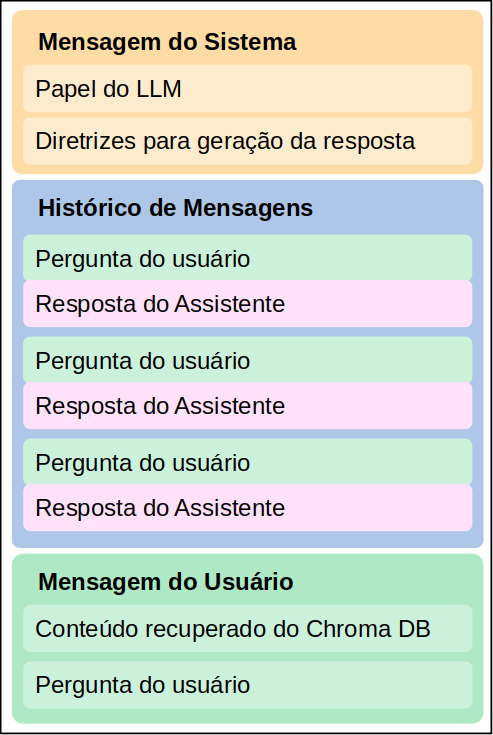
\includegraphics[width=0.5\linewidth]{Imagens/pilha-mensagem-ollama.png}
    \caption{Estrutura da mensagem enviada ao Ollama}
    Fonte: autoria própria
    \label{fig:pilha-mensagem-ollama}
\end{figure}


De forma a direcionar o comportamento dos \ac{LLM}s na geração das respostas, cada requisição feita à API utiliza uma mensagem de sistema fixa, bem como um modelo de \textit{prompt} com uma estrutura pré-definida (ver Figura \ref{fig:pilha-mensagem-ollama}), alterando somente a pergunta feita e o teor dos documentos em que a resposta deve se basear. Assim, os dados enviados à API têm a seguinte estrutura:

\begin{itemize}
    \item \textbf{Papel do \ac{LLM}}: Definição do papel que o modelo deve assumir, cujo teor é  
    \begin{quote}
    {
        \footnotesize
        \ttfamily
        \raggedright
        \sloppy
        ``Alern e ALRN significam Assembleia Legislativa do Estado do Rio Grande do Norte.
        
        Você é um assistente que responde a dúvidas de servidores da Alern sobre o regimento interno da Alern, o regime jurídico dos servidores estaduais do RN, bem como resoluções da Alern.
        
        Assuma um tom formal, porém caloroso, com gentileza nas respostas.
        
        Utilize palavras e termos que sejam claros, autoexplicativos e linguagem simples, próximo do que o cidadão comum utiliza.
        
        Responda utilizando o mesmo idioma em que a pergunta foi feita.'';
    }
    \end{quote}
    \item \textbf{Diretrizes de Geração}: Orientações a serem seguidas pelo \ac{LLM} na geração da resposta, sendo afixado como

        \begin{quote}
        {
        \begin{minipage}{\dimexpr\linewidth-2em}
        \setlength{\rightskip}{0.7em}
        \footnotesize
        \ttfamily
        \raggedright
        \sloppy
        ``Responda utilizando o mesmo idioma que foi usado na pergunta.
        
        Use as informações dos DOCUMENTOS fornecidos para gerar uma resposta clara para a PERGUNTA.
        
        Na resposta, não mencione que foi fornecido documentos de referência.
        
        Cite os nomes dos DOCUMENTOS e números dos artigos em que a resposta se baseia.
        
        A resposta não deve ter saudação, vocativo, nem qualquer tipo de introdução que dê a entender que houve interação anterior.
        
        As respostas dadas devem ser específicas para a pergunta atual, usando o histórico somente para fim de contexto.
        
        Se você não souber a resposta, assuma um tom gentil e diga que não tem \\ informações suficientes para responder.
        
        Caso a pergunta seja sobre temas que não envolvam busca de informação na documentação da Alern, educadamente se recure a responder. Em nenhuma circunstância escreva texto que incite violência ou comportamento criminoso e inadequado.'';
        \end{minipage}
        }
        \end{quote}
    \item \textbf{Histórico}: uma lista com o teor das mensagens trocadas anteriormente entre o usuário e o assistente. Dado que cada \ac{LLM} possui uma limitação no número máximo de \textit{tokens} dos \textit{prompts} por eles processados, apenas uma fração do conteúdo recebido pelo \ac{LLM} é incluída no histórico, sendo correspondente às 5 mais recentes interações do usuário com o assistente -- cinco pares pergunta-resposta. Nesse recorte, não estão contidos os conteúdos recuperados do banco vetorial (os quais serviram de base para a geração da resposta do Assistente), de sorte que apenas as perguntas feitas pelos usuários e as respostas dadas pela ferramenta são mantidas no histórico.
    
    \item \textbf{\textit{Prompt} do usuário}: texto formado pelo conteúdo dos documentos a serem utilizados para a geração da resposta e pela pergunta a ser respondida pelo \ac{LLM}. A Figura \ref{fig:prompt-usuario} mostra um exemplo de um \textit{prompt} em seu formato final.
\end{itemize}

\begin{figure}[H]
    \centering
    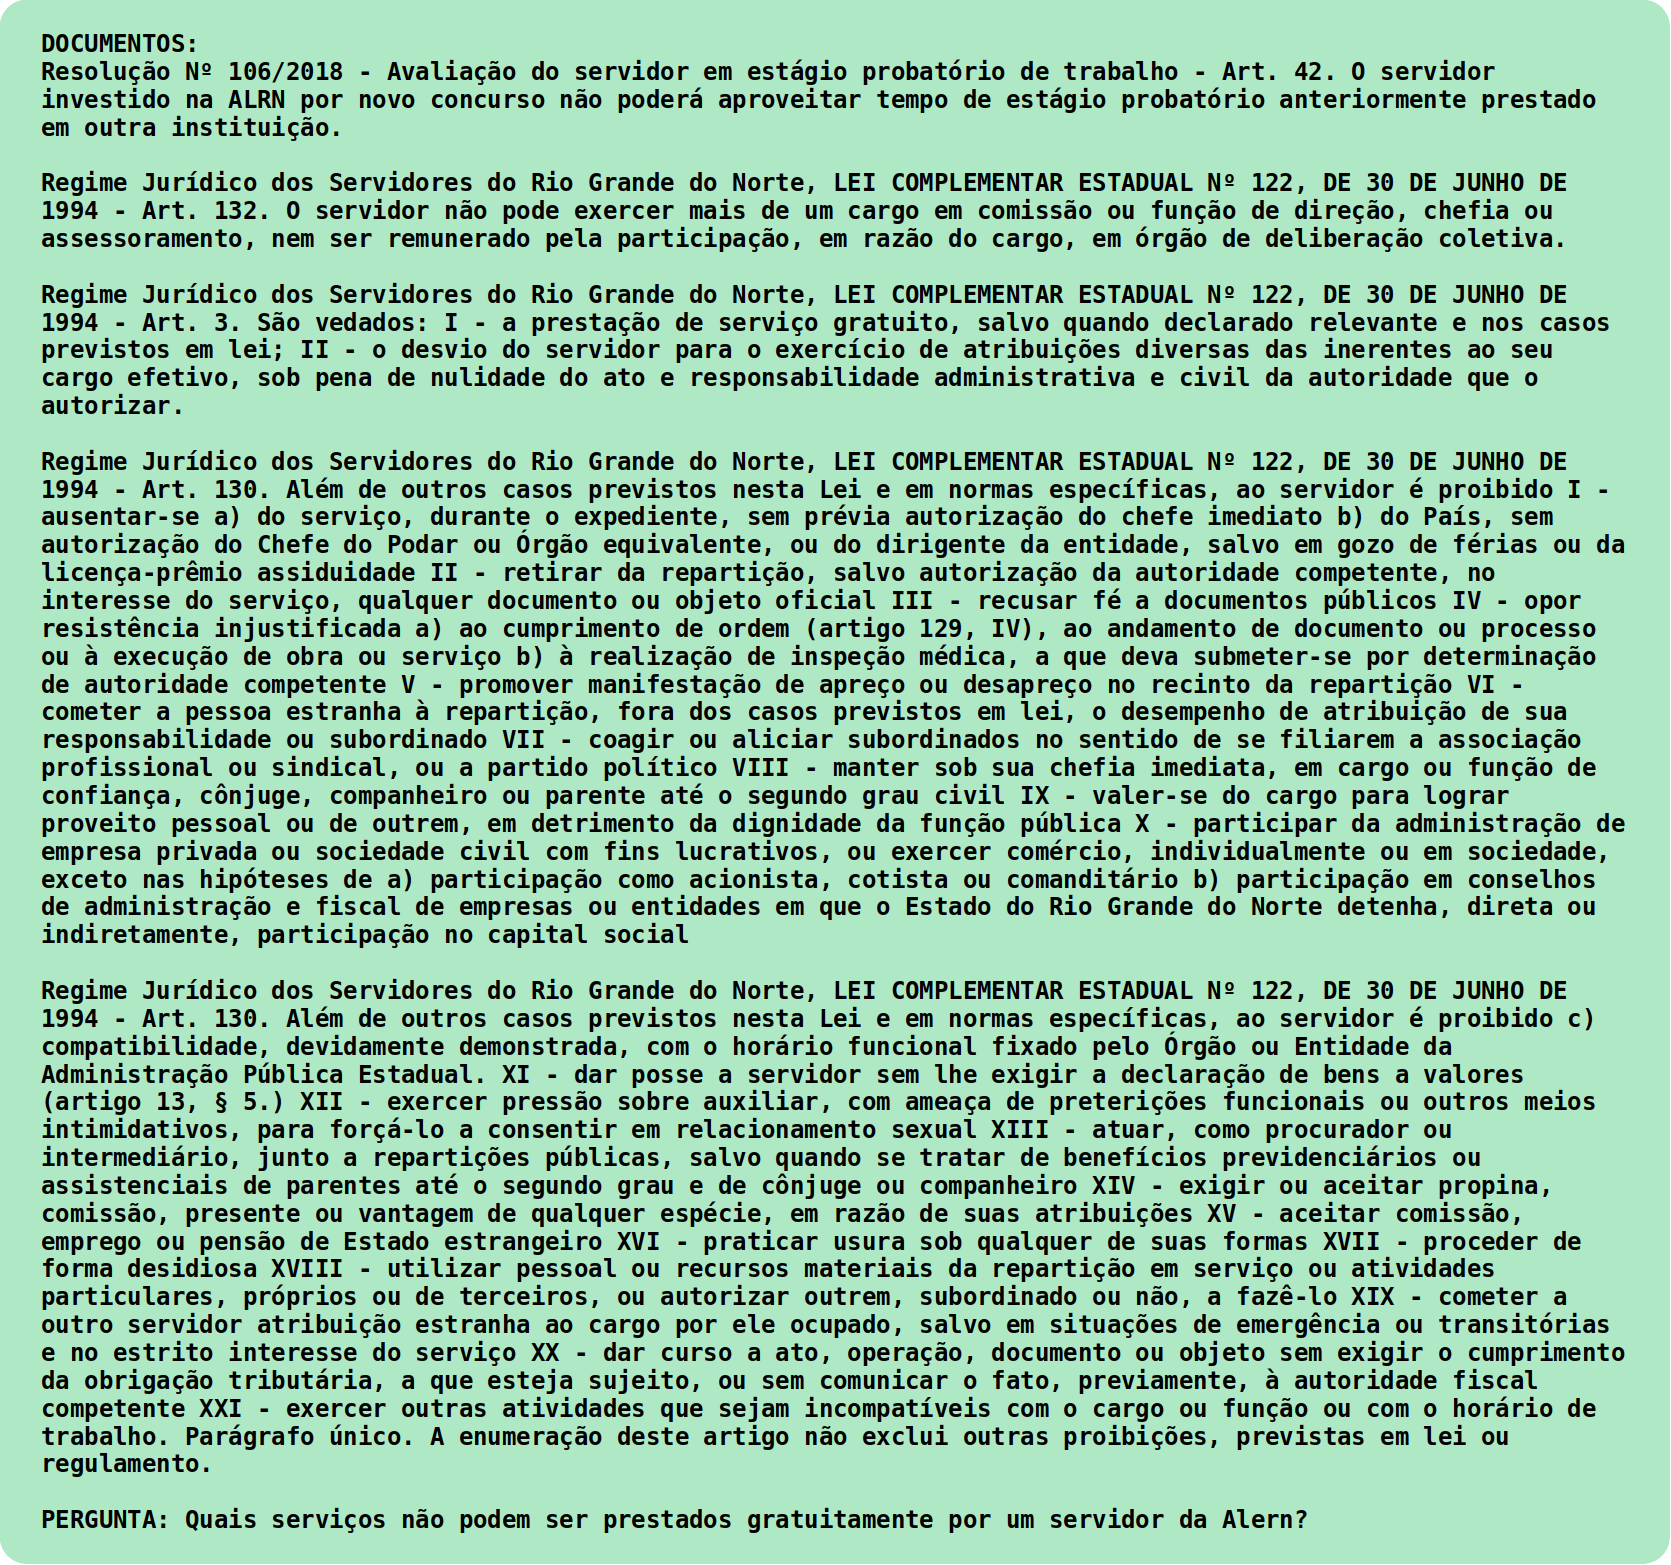
\includegraphics[width=1\linewidth]{Imagens/prompt-usuario.png}
    \caption{Estrutura do \textit{prompt} de usuário}
    Fonte: autoria própria
    \label{fig:prompt-usuario}
\end{figure}

\section{API Gerenciadora de Fluxo}
\label{sec:Metodologia.4}

A integração de todos os serviços oferecidos pelas camadas mencionadas é realizada por uma API gerenciadora de fluxo (utilizando a biblioteca FastAPI, na linguagem Python), que se encarrega de receber requisições de alguma interface de usuário, com as perguntas a serem utilizadas como critérios de consulta e acionar os serviços das outras camadas para a geração da resposta. Após receber os dados resultantes de cada um dos serviços nas fases intermediárias do processo inteiro, eles são formatados e preparados para serem direcionados ao elemento seguinte, até, finalmente, encaminhar à interface de usuário o produto final, na forma de uma resposta, com uma lista de documentos que lhe dão suporte.

A Figura \ref{fig:diag-atividade-assist-busca} demonstra o fluxo inteiro do processo como um todo.

\begin{figure}[H]
    \centering
    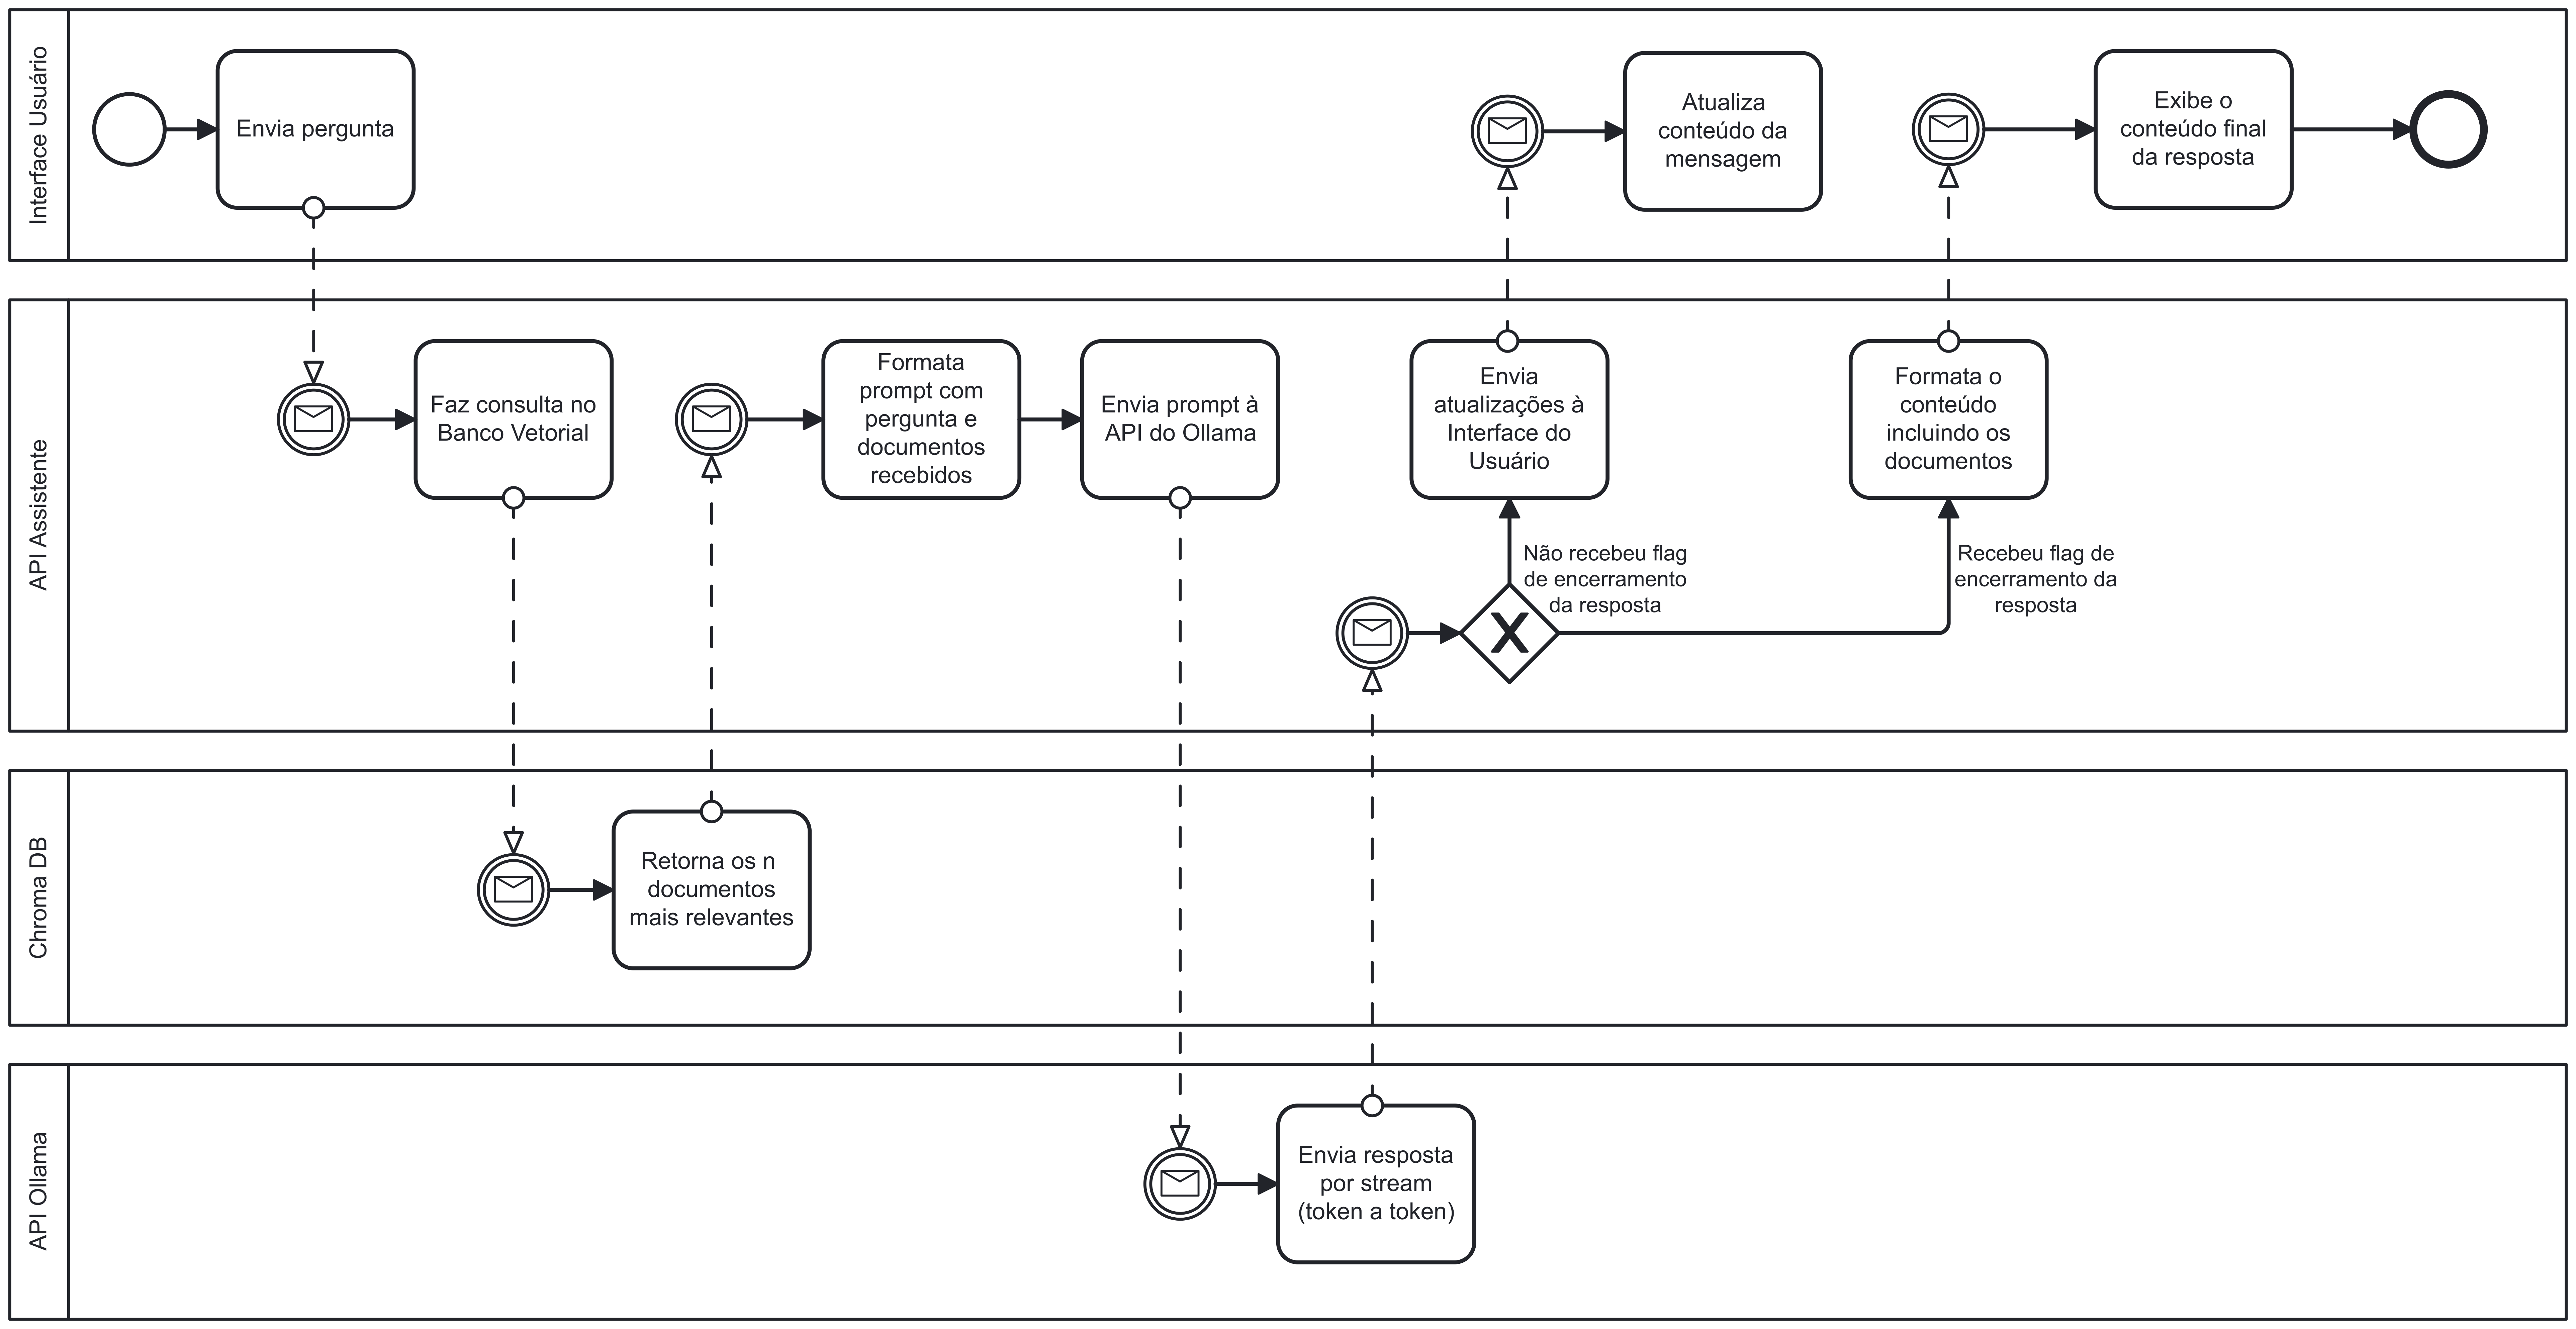
\includegraphics[width=1\linewidth]{Imagens/diagram.png}
    \caption{Diagrama de Atividades do Assistente de Busca}
    Fonte: autoria própria
    \label{fig:diag-atividade-assist-busca}
\end{figure}

Além de incluir a pergunta, a resposta e o conjunto de documentos que foram utilizados na composição do \textit{prompt} enviado ao \ac{LLM}, a API Gerenciadora de Fluxo coleta dados a respeito do processo como um todo (tempo levado na execução de cada etapa, métricas utilizadas, dentre outros) e os inclui na resposta devolvida ao usuário. Também cabe a esse elemento garantir persistência de dados sobre cada uma das interações realizadas, permitindo que, a posteriori, sejam analisados e utilizados para refinamento do processo e da estrutura proposta. Por conveniência e compatibilidade com as estruturas de armazenamento já existentes na Alern, os dados das interações serão salvos em bancos Relacionais.

\section{Interface de Usuário}
\label{sec:Metodologia.5}

Dado o objetivo deste estudo, foi definida uma página \textit{web} como interface de usuário -- considerando sua simplicidade de desenvolvimento e implementação -- nos moldes de uma aplicação de envio/recebimento de mensagens de texto, como é o mais comum ao se desenhar uma ferramenta de \textit{chatbot}, conforme visto na Figura \ref{fig:interface-assist-busca}.

\begin{figure}[H]
    \centering
    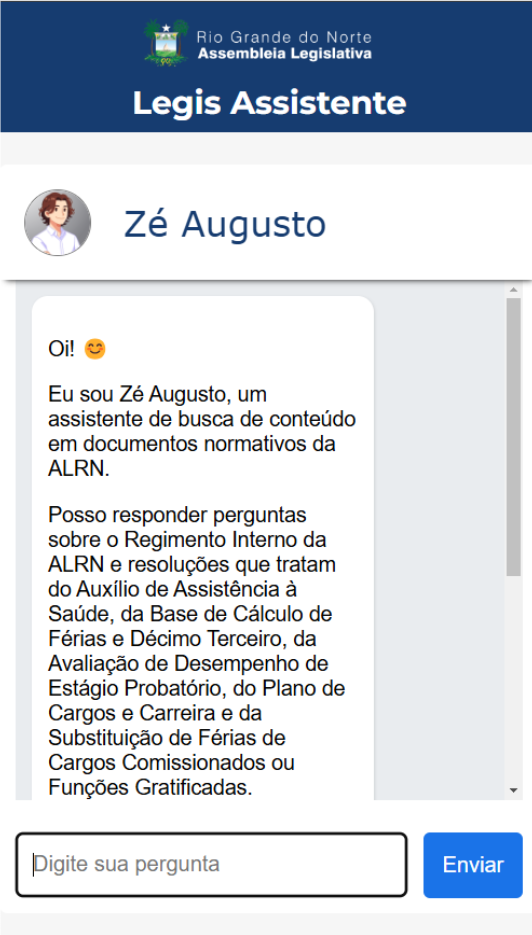
\includegraphics[width=0.5\linewidth]{Imagens/interface_usuario.png}
    \caption{Interface de Usuário Inicial do Assistente de Busca}
    Fonte: autoria própria
    \label{fig:interface-assist-busca}
\end{figure}

A opção foi feita por manter uma interface limpa e minimalista, restringindo-se somente ao campo de envio de mensagens do usuário, bem como uma área superior com a exibição das mensagens enviadas e recebidas. Para isso, utilizamos uma página HTML simples, sem utilização de qualquer \textit{framework} ou tecnologia mais elaborada, valendo-se de Javascript para estabelecer comunicação com a API, receber os resultados e alterar elementos na interface em si, à medida que o usuário interage com a ferramenta.

Quando cada resposta é recebida, o usuário pode escolher avaliar a resposta recebida como satisfatória, como uma resposta ruim, ou ainda reportar a resposta como contendo conteúdo indevido -- mostrado na Figura \ref{fig:interface-assist-busca-resposta}. As avaliações dos usuários serão utilizadas para análise e como recursos para, eventualmente, criar um conjunto de dados que permita futuro refinamento dos modelos utilizados.

\begin{figure}[H]
    \centering
    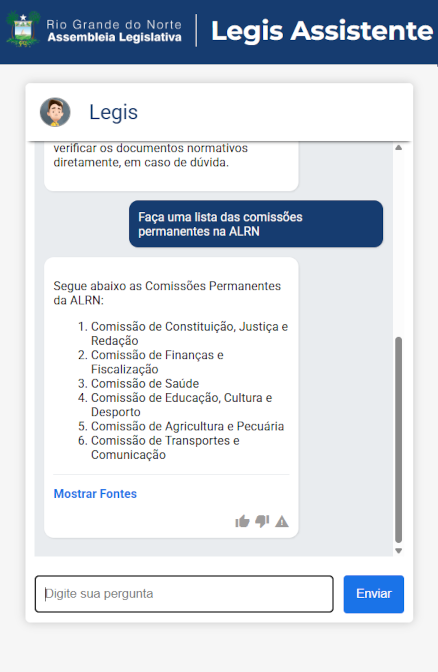
\includegraphics[width=0.5\linewidth]{Imagens/interface_usuario_resposta.png}
    \caption{Interface de Usuário do Assistente de Busca com Resposta}
    Fonte: autoria própria
    \label{fig:interface-assist-busca-resposta}
\end{figure}

Optamos, para fins de simplicidade, manter uma abordagem em que as perguntas e respostas do usuário são voláteis, de forma que, para o usuário, não há continuidade entre as sessões de uso. Cada sessão (marcada pelo carregamento da página de \textit{chat}) se inicia com um histórico limpo de interações, de forma que a persistência dos dados das interações é feita e mantida somente para fins de avaliação, sem ser retomada pelo usuário em qualquer momento futuro.

A mecânica de consulta consiste apenas de uma solicitação realizada à API de gerenciamento do fluxo de informações, por meio de requisição HTTP, que envia a pergunta ou frase de consulta a ser utilizada como critérios de busca no banco vetorial, bem como um vetor de \textit{embeddings} contendo os dados das interações mais recentes, o qual será utilizado como informação do contexto, junto ao \ac{LLM}, de forma a manter um senso de continuidade no \textit{chat}.

\section{Medição dos Resultados}
\label{sec:Metodologia.6}
Considerando a natureza da tarefa a que se propõe a aplicação objeto deste estudo (especificamente o resultado final do processo), entende-se que uma avaliação criteriosa feita por um humano seria o adequado para aferir se a resposta dada é satisfatória para a pergunta ou consulta realizada. Em um cenário ideal, esse avaliador também teria conhecimento aprofundado do domínio no qual a aplicação atua, de forma a garantir que não somente a resposta é coerente, mas também se o conhecimento que ela se pretende a suprir está acurado. Esse tipo de avaliação, contudo, por sua própria natureza, demanda tempo -- que acaba por ser ainda mais custoso, por envolver um especialista numa área de domínio -- e se mostra pouco escalável, dado que o volume de amostras a serem avaliadas fica restrito à disponibilidade de avaliadores.

Ainda assim, uma das formas de avaliação do desempenho do Assistente de Busca como um todo a que pretendemos é do tipo qualitativa, baseando-se no parecer dado por especialistas nas matérias de que trata o corpus documental que foi selecionado para o desenvolvimento e testes. O grupo de especialistas inclui, dentre outros, servidores atuantes na \ac{CDHO}, da Assembleia Legislativa do Rio Grande do Norte, dado que a prática diária de suas atividades os torna familiarizados com os meandros das Resoluções e definições regimentais contidas na seleção de documentos abordada neste estudo.

Assim, interagiriam os especialistas com a interface de usuário, inserindo perguntas sobre aspectos relevantes cobertos pelos atos normativos no conjunto de documentos selecionados. As interações dos especialistas não serão guiadas ou direcionadas, de forma que as perguntas feitas sejam orgânicas e o mais próximo possível do tipo de uso que o Assistente de Busca terá após sua implementação e disponibilização. Os avaliadores observarão as respostas geradas, aferindo quantitativamente a sua exatidão e fornecendo eles mesmos um texto breve com o teor do que deveria ser a resposta ideal.

Os dados coletados da interação serão armazenados para análise posterior, e, a depender da quantidade de dados coletados, utilizados para eventual refinamento e ajuste fino dos modelos que servem de base para as camadas da ferramenta.

Não obstante, há um aspecto relevante a ser considerado, o qual potencialmente emergirá das condições de avaliação propostas. Dado que os especialistas farão perguntas sem direcionamento, é improvável que o conjunto total de perguntas submetidas ao Assistente de Busca tenha uma variedade grande o suficiente para abordar toda a amplitude de matérias presentes nos documentos. Perguntas repetidas, aspectos sobre os quais não lhes ocorrerá perguntar, assuntos cuja natureza seja considerada demasiadamente óbvia para questionamento, entre outros, são alguns dos problemas cuja ocorrência pode ser prevista com algum grau de confiança.

No que concerne à avaliação realizada pelos especialistas, além da possível falta de cobertura das perguntas feitas, há outro ponto delicado cuja abordagem é relevante. Dado que a avaliação dos especialistas em relação ao Assistente, da forma como descrita, se debruça somente sobre o resultado final do processo -- a resposta -- a identificação de possíveis elementos responsáveis pela qualidade aquém da esperada se torna menos efetiva, posto que são perdidas informações dos processos intermediários da geração da resposta. Nessas condições, embora seja possível a identificação de respostas inadequadas, os dados não são suficientes para determinar se a falha ocorreu na recuperação dos documentos junto ao banco vetorial ou se a resposta gerada pelo \textit{Llama} foi incorreta, mesmo com as informações adequadas disponíveis.

Com o fim de mitigar esses dois problemas apontados, serão feitas avaliações utilizando uma abordagem diferente, buscando garantir cobertura tanto da totalidade do conteúdo no banco vetorial quanto a verificação de resultados intermediários que são elementos base para a geração da resposta final. Analisaremos o seguinte:

\begin{itemize}
    \item o quanto os resultados das buscas no banco vetorial são pertinentes às perguntas, comparando os modelos (avaliação automatizada quantitativa);
    \item o tempo de execução/latência nas buscas no banco vetorial (avaliação automatizada quantitativa);
    \item a qualidade da resposta final gerada pelo Assistente (avaliações humana qualitativa e automatizada quantitativa).
\end{itemize}

De forma a alcançar esse objetivo, com base no conteúdo existente no banco vetorial, geraremos sinteticamente um conjunto de dados que permitirá explorar cada uma das etapas do processo de geração de respostas, possibilitando avaliar os resultados intermediários e finais da aplicação. Especificamente, esse conjunto terá, para cada um dos fragmentos inclusos no banco vetorial, o seguinte:

\begin{enumerate}
    \item uma lista de perguntas baseadas no conteúdo do fragmento;
    \item uma lista de respostas de referência para cada uma dessas perguntas, compostas por trechos do respectivo fragmento;
    \item um conjunto com os 10 fragmentos com maior similaridade semântica com a pergunta, obtidos do banco vetorial;
    \item uma resposta final para a pergunta, gerada pelo Assistente.
\end{enumerate}

A abordagem, portanto, para avaliar o grau de eficácia dos modelos de \textit{embeddings} consiste em, dado que sabemos qual o fragmento original que foi utilizado para geração de cada uma das perguntas, analisar seu respectivo conjunto de fragmentos de documentos recuperados do banco vetorial e observar se o fragmento original é um de seus elementos. No que concerne à validação da resposta final gerada, pode ser utilizada a métrica \textit{BERTScore} de similaridade entre a resposta final e a resposta de referência.

Como meio de automação da tarefa de geração do conteúdo base, tomamos a decisão de utilizar um segundo \ac{LLM} parametrizado com o objetivo específico de gerar tanto o conjunto de perguntas quanto o de respostas. Com a ciência de que, na prática, teremos um conteúdo gerado por um \ac{LLM} (a resposta final) sendo avaliado com base em um conteúdo também gerado por um \ac{LLM} (a resposta de referência), definimos, como forma de prover um mínimo de independência, que utilizaríamos modelos diferentes para a execução de cada uma das tarefas. Uma vez que optamos pelo \textit{Llama3.1} como \ac{LLM} a integrar a arquitetura do Assistente de Busca, adotamos o \textit{GPT-4o} \cite{GPT4o:1} para a geração das perguntas e respostas -- tanto por ser não relacionado com os modelos sendo avaliados (\textit{Llama3.1} e \textit{DeepSeek-r1}), como também pela reconhecida qualidade de conteúdo gerado.


\subsection{Processo de Geração dos Dados de Teste}
\label{subsec:Metodologia.6.1}


Para a efetiva geração dos dados a serem utilizados com testes e avaliações, cada um dos fragmentos documentais foi utilizado em um \textit{prompt} de geração de conteúdo a ser processado por uma instância do modelo \textit{GPT-4o}, da OpenAI (por meio da API fornecida pela OpenAI, para consulta externa). O teor do \textit{prompt} é como segue:

\begin{quote}
{
    \footnotesize
    \ttfamily
    \raggedright
    \sloppy
    Considere o texto a seguir, que é um artigo de uma lei:
    
    \{artigo\}
    
    Agora extraia as informações do artigo e gere perguntas que possam ser respondidas com base no conteúdo textual do artigo.
    
    Além disso, formule a resposta com base no artigo e em nenhuma outra fonte. As perguntas e respostas serão utilizadas para treinamento e \textit{finetuning} de um LLM. Siga as seguintes diretrizes para gerar as perguntas e respostas:

    Considere o texto recebido e identifique informações significativas;
    
    Com base nas informações, crie pelo menos 3 perguntas que possam ser respondidas com base no conteúdo do texto;
    
    Caso o texto fornecido não tenha informação a partir da qual seja possível criar perguntas relevantes, deve ser retornado um objeto vazio;
    
    As perguntas devem ser claras, diretas, e específicas;
    
    As perguntas podem ter sinônimos ou termos aproximados do texto base, mas devem ser possível de ser respondidas pelo texto fornecido;
    
    Para cada pergunta, formule uma resposta usando como base o conteúdo do artigo, sem utilizar qualquer outro conhecimento que você disponha.

    Cada pergunta será aceitável somente se:

    * Estiver relacionada aos assuntos pertinentes ao artigo apresentado
    
    * For uma pergunta relevante, semelhante ao que seria perguntado por uma pessoa com dúvida
    
    * Puder ser respondida usando o fragmento apresentado

    O resultado deve ser em formato estruturado, em formato JSON, sendo uma lista de objetos assim:
    
    [\{``pergunta'': ``texto da pergunta'', ``resposta'':``texto da resposta''\},
    
     \{``pergunta'': ``texto da pergunta'', ``resposta'':``texto da resposta''\}]
    
    Não deve haver nenhum outro texto, apenas a lista.

    Um exemplo de como devem ser geradas as perguntas:

    Exemplo de texto base:
    
    ``Art. 1º A Assembleia Legislativa é composta de Deputados, representantes do povo norte-rio-grandense, eleitos, na forma da lei, para mandato de 4 (quatro) anos.''

    Resultado aceitável:
    
        [\{``pergunta'': ``A Assembleia Legislativa é formada pelo que?'', ``resposta'': ``A Assembleia Legislativa é composta por Deputados, que são eleitos pelo do povo norte-rio-grandense e os representam.'',\},
            
        \{``pergunta": ``O que é um Deputado?",``resposta": ``Um Deputado é um representante eleito do povo, possuindo mandato de quatro anos.''\},
        \{``pergunta'': ``Quanto tempo dura um mandato?'',``resposta'': ``Um mandato dura pelo período de quatro anos.''\}]

    Caso o texto não tenha conteúdo relevante, o resultado deve ser um objeto vazio \{\}.

    Vamos começar?
}
\end{quote}

O resultado gerado pelo \textit{GPT-4o} foi analisado com fins de assegurar sua correção em termos de formato JSON, para garantir que o arquivo estivesse válido e pudesse ser usado no processo de avaliação. Dessa forma, cada fragmento no banco vetorial recebeu um conjunto de perguntas, acompanhado de suas respectivas respostas, geradas com base no texto do próprio fragmento, sendo, portanto, ambas diretamente relacionadas ao conteúdo que lhes deu origem. Essas respostas para as perguntas elaboradas serão utilizadas como resposta de referência ao se avaliar a qualidade do conteúdo das respostas finais geradas pelo \ac{LLM} integrante do Assistente de Busca, por meio do \textit{BERTScore}, conforme descrito na Seção \ref{subsec:Resultados.2.2}. A Figura \ref{fig:geracao-perguntas} resume o processo de geração das perguntas e respostas.

\begin{figure}[H]
    \centering
    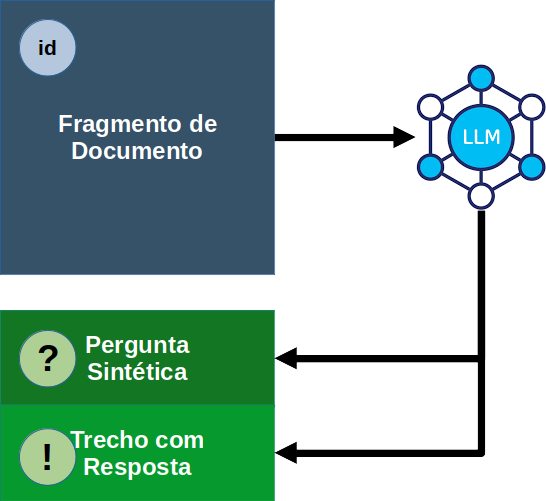
\includegraphics[width=0.5\linewidth]{Imagens/geracao-perguntas.png}
    \caption{Geração de pares pergunta-resposta por meio de LLM}
    Fonte: autoria própria
    \label{fig:geracao-perguntas}
\end{figure}

Após a geração do conjunto de perguntas ``sintéticas'' para cada fragmento, cada pergunta foi usada para realizar buscas no banco vetorial com o objetivo de identificar documentos semanticamente semelhantes. Como resultado, para cada pergunta associada a um fragmento, foi gerado um conjunto de documentos considerados semanticamente próximos (ver Figura \ref{fig:recuperacao-fragmentos}).

\begin{figure}[H]
    \centering
    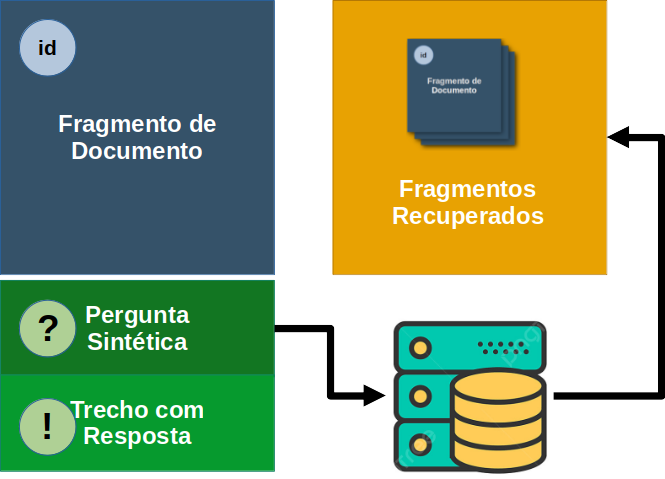
\includegraphics[width=0.5\linewidth]{Imagens/recuperacao-fragmentos.png}
    \caption{Recuperação de documentos do Banco Vetorial}
    Fonte: autoria própria
    \label{fig:recuperacao-fragmentos}
\end{figure}

Com as perguntas e seus correspondentes conjuntos de documentos relevantes, foi possível utilizar esses materiais, conforme detalhado na Seção \ref{sec:Metodologia.3}, para criar um \textit{prompt} e solicitar ao \textit{Llama} que gerasse uma resposta completa baseada na seleção de documentos. Esse processo emula a dinâmica seguida pelo Assistente de Busca durante seu uso comum pelos usuários, simulando uma interação que visa fornecer respostas completas e relevantes a partir de consultas realizadas (Figura \ref{fig:geracao-respostas}).

\begin{figure}[H]
    \centering
    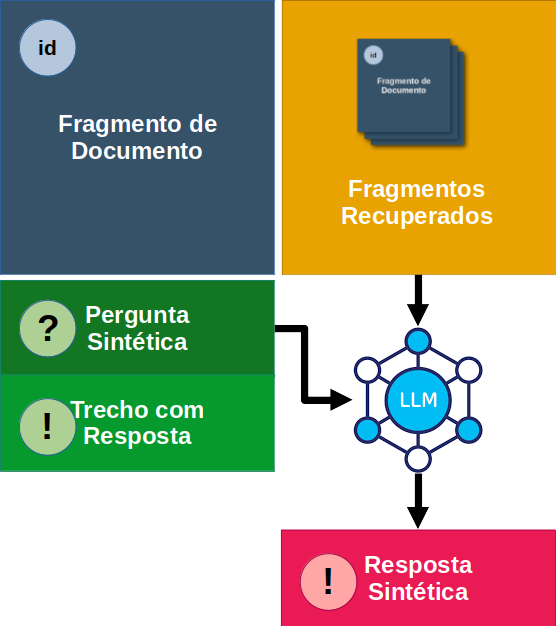
\includegraphics[width=0.5\linewidth]{Imagens/geracao-respostas.png}
    \caption{Recuperação de documentos do Banco Vetorial}
    Fonte: autoria própria
    \label{fig:geracao-respostas}
\end{figure}

Havendo sido concluídas todas essas etapas, foi possível obter, para cada pergunta gerada sinteticamente, uma estrutura de dados como a apresentada na Tabela \ref{tab:dados-sinteticos}. Esses dados gerados possibilitam não somente a abordagem de mitigação dos problemas apontados, como também a realização de uma avaliação preliminar também automatizada, com foco nas duas etapas de geração das respostas: a recuperação de documentos por similaridade, junto ao banco vetorial, e a elaboração do texto final da resposta feita pelo \textit{Llama}, com base no teor dos documentos selecionados.

\begin{table}[H]
    \caption{Estrutura dos dados sintéticos gerados para cada fragmento}
    \centering
    \begin{tabular}{ l p{10cm} }
         \hline
         \textbf{Informação} & \textbf{Descrição} \\  
         \hline
         Id & Identificador do fragmento usado para gerar a pergunta \\
         Pergunta & Pergunta gerada pelo \textit{GPT-4} com base no fragmento \\
         Resposta & Proposta de resposta do \textit{GPT-4} para a pergunta gerada \\
         Fragmentos & Lista de fragmentos relevantes recuperados do banco de vetores \\
         Resposta \textit{Llama} & Resposta gerada pelo \textit{Llama} com base na pergunta e nos fragmentos relevantes \\
         \hline
    \end{tabular}
    
    Fonte: O autor (2024)
    \label{tab:dados-sinteticos}
\end{table}

\subsection{Avaliação da Recuperação de Conteúdo (\textit{Retrieval})}
\label{subsec:Metodologia.6.2}
Como forma de avaliar a recuperação dos fragmentos realizada pelo banco de vetores, é possível lançar mão de dois campos presentes na estrutura de dados apresentada na Tabela \ref{tab:dados-sinteticos}, a saber: Id (que contém o identificador do fragmento utilizado para gerar a pergunta) e Fragmentos (que contém os fragmentos recuperados do banco vetorial). Consideremos que cada pergunta foi gerada com base no conteúdo de um fragmento específico de documento. A partir disso, é possível assumir que é natural que exista uma similaridade entre o teor da pergunta e o do fragmento original. Pelos mesmos motivos, também é esperado que, entre os fragmento recuperados na avaliação de semelhança semântica, esteja incluído o próprio fragmento que serviu de base para a criação da pergunta.

Adicionalmente, considerando que é possível recuperar o conteúdo do fragmento base -- gerador da pergunta -- bem como obter o texto dos fragmentos retornados pelo banco vetorial, existe uma abordagem alternativa à verificação do grau de similaridade entre a pergunta e os fragmentos retornados. Em vez de se lançar mão da pergunta, utiliza-se como parâmetro de avaliação a similaridade entre o conteúdo do fragmento base com os textos dos fragmentos retornados.

Em suma, para cada pergunta sintética utilizada, avaliaremos se o id do fragmento original, utilizado para gerar a pergunta, figura entre os ids do conjunto de fragmentos retornados do banco vetorial. Consideraremos bem sucedida a execução do processo caso haja a presença do id alvo no conjunto de fragmentos recuperados.

Dentro do conjunto textual, os documentos articulados correspondem a textos normativos sobre temas específicos, de forma que há muito pouco de sobreposição de temas entre eles. O documento não articulado (Manual de Processo Legislativo -- listado como documento 12 nas Tabelas \ref{tab:descricao-documentos-1} e \ref{tab:descricao-documentos-1}), contudo, aborda muito do que é tratado na Resolução Nº 031/2021 (O Regimento Interno da Alern, presente nas Tabelas \ref{tab:descricao-documentos-1} e \ref{tab:descricao-documentos-1} como documento 2), detalhando os meandros do processo legislativo. Portanto, é natural que haja uma grande interseção de assuntos neles presentes.

Como forma de averiguar o desempenho dos modelos diante de variados cenários de documentos, realizaremos os testes com três configurações distintas, em termos de diversidade das temáticas abordadas pelos documentos, bem como de suas estruturas. 

\begin{itemize}
    \item Recuperação dos fragmentos \textit{somente dos documentos articulados}, cada um deles referente a um assunto exclusivo, não majoritariamente abordado por outros documentos;
    \item Recuperação dos fragmentos de documentos articulados e do documento estruturado (Manual de Processo Legislativo) -- o que inclui uma quantidade considerável de sobreposição de conteúdo entre os elementos; e
    \item Recuperação de fragmentos de um conjunto de dados textuais sem qualquer restrição de sobreposição temática, utilizando o conteúdo publicado na página de notícias da Alern, mantida pela Coordenadoria de Comunicação da Casa, para fins de comparação de performance.
\end{itemize} 


O conjunto de textos da terceira abordagem é composto por mais de mil notícias relacionadas especificamente a sessões ordinárias e reuniões de comissões, as quais tratam de sumarizar os pontos mais relevantes das discussões travadas e das propostas apresentadas pelos parlamentares. São textos lineares e não possuem qualquer tipo de estrutura ou hierarquia definida -- salvo pela existência de um título, que dá um indicativo do seu conteúdo. Então como estratégia de particionamento, nos limitamos a dividir as notícias por parágrafo, para ser o conjunto de fragmentos e prepusemos o texto do título da notícia, como forma de lhes garantir um mínimo de contexto. A Tabela \ref{tab:descricao-noticias} descreve os aspectos da do conjunto de dados.

\begin{table}[H]
    \caption{Descrição do dataset de notícias}
    \centering
    \begin{tabular}{ l r }
        \hline
        \bfseries Característica & \bfseries Valor \\
        \hline
        Media de Fragmentos por notícia & 5,6 \\
        Media de Tamanho & 299,8 \\
        Quantidade de Notícias & 1.436 \\
        Quantidade de Fragmentos & 8.044 \\
        \hline
    \end{tabular}
    
    Fonte: O autor (2025)
    \label{tab:descricao-noticias}
\end{table}

\subsection{Avaliação das Respostas Geradas pelo LLM}
\label{subsec:Metodologia.6.3}
A avaliação da qualidade das respostas geradas pelo \ac{LLM} é um aspecto fundamental para garantir a eficácia e a confiabilidade das respostas geradas com base nos documentos recuperados. Uma avaliação eficaz não deve se limitar a quantificar a similaridade entre a resposta gerada e a pergunta original. Em vez disso, foca na capacidade de a resposta satisfazer as expectativas informacionais do usuário. Essa abordagem assegura que as respostas não apenas sejam relevantes em um sentido superficial, mas que realmente atendam aos critérios de completude e precisão em relação ao corpus documental utilizado.

Embora a similaridade entre a pergunta e a resposta seja uma métrica viável, demonstra-se insuficiente para avaliar a qualidade da resposta em um nível mais profundo. A análise de proximidade semântica da resposta em relação à pergunta não garante que a resposta abranja de forma adequada o contexto e o conteúdo desejado pelo próprio fato de que uma resposta, por definição, deve conter informações inexistentes na pergunta. Portanto, a avaliação deve ir além da correspondência superficial e considerar o quão bem a resposta aborda e resolve a questão apresentada.

\subsubsection{Avaliação Automatizada}
\label{subsubsec:Metodologia.6.3.1}
Para avaliar a qualidade das respostas em termos de satisfação da pergunta, ferramentas como o BERTScore, proposto por \citeonline{BERTScore:1}, abordado na Seção \ref{sec:Teorico.7}, se mostram úteis. Sua aplicação em sistemas de \ac{RAG} oferece uma maneira objetiva de quantificar o desempenho dos \ac{LLM}s no que tange à satisfatoriedade de suas respostas às perguntas. Essa métrica considera a semelhança semântica e permite identificar se uma resposta contém informações relevantes e está alinhada com o que foi solicitado pela pergunta. Assim, como métrica de avaliação da resposta final gerada utilizamos o BERTScore sobre a resposta, gerada para cada uma das perguntas sintéticas disponíveis, em relação à sua respectiva resposta de referência (ver Seção \ref{subsec:Metodologia.6.1}), dado que este contribui para a validação da qualidade da resposta gerada, não apenas em termos de similaridade de palavras, mas em relação à precisão e completude, características essenciais para a construção de sistemas de perguntas e respostas de alta qualidade. Como resultado, se alcança uma medida mais robusta de como a resposta aborda de maneira contextualizada a pergunta, indo além da análise de correspondência lexical.

Cabe pontuar, contudo, que o BERTScore servirá tão somente como uma ferramenta quantitativa de avaliação das respostas, motivo pelo qual utilizaremos avaliação humana para dar conta de aspectos mais qualitativos das respostas.

\subsubsection{Avaliação Humana}
\label{subsubsec:Metodologia.6.3.2}
A avaliação humana da qualidade das respostas geradas se debruçará sobre dois aspectos do produto final da aplicação \ac{RAG}: as características estruturais do texto gerado e o conteúdo gerado, em si.

Inicialmente, será conduzida uma investigação exploratória sobre o material produzido pelos modelos, com o objetivo de obter uma visão panorâmica e destacar eventuais irregularidades evidentes, perceptíveis sem necessidade de exame detalhado. Entre esses aspectos, serão observados o comprimento das respostas, a lógica de suas construções textuais, a uniformidade no uso do idioma, bem como outras possíveis anomalias que possam surgir no decorrer da análise.

Após isso, uma análise mais estruturada e sistemática será feita das respostas, baseando-se em perguntas orgânicas -- feitas por avaliadores humanos, em vez de perguntas sintéticas. Para isso, contaremos com a ajuda de servidores da \ac{Alern}, aos quais será solicitado que elaborem perguntas que possam ser respondidas através de conteúdo presente nos documentos integrantes do nosso conjunto de dados, juntamente com suas respectivas respostas. As perguntas serão utilizadas para gerar respostas, seguindo todo o fluxo da aplicação \ac{RAG} (recuperação de documentos, formatação do conteúdo, injeção do resultado para criação de um \textit{prompt} e sua submissão à API da ferramenta de execução de \ac{LLM}s, para geração da resposta). Ao todo, 4 servidores colaborarão para esta parte do processo, gerando um total de 20 perguntas.

Após isso, as respostas serão apresentadas aos avaliadores, os quais receberão direcionamento para avaliar as respostas sob os seguintes critérios:

\begin{itemize}
    \item Corretude: avalia o quão correta a resposta está, tanto em termos de não apresentar informações falsas, quanto em termos de responder a pergunta;
    \item Coerência: avalia o quanto o teor da resposta (correta ou não) está escrito de forma coerente -- apresenta sentido coerente, incluindo mostrar consistência no idioma utilizado;
    \item Gramática e Ortografia: avalia se as palavras utilizadas estão corretamente grafadas e se as frases têm escrita gramaticalmente correta;
    \item Adequação: avalia se o nível de escrita apresenta vocabulário adequado à compreensão do usuário comum, conforme definido nas diretrizes passadas via \textit{prompt}.
\end{itemize}

Para cada um dos critérios, o avaliador deverá atribuir um valor de 0 nos casos em que a pergunta gerada tiver um desempenho ``ruim'', 1 para um desempenho ``aceitável'' ou 2 para um desempenho ``bom'' / plenamente satisfatório. Para cada um dos modelos utilizados, será calculado o somatório dos pontos em cada um dos critérios e a porcentagem da pontuação máxima possível de ser alcançada.

Os resultados das avaliações humanas serão, após o processo, compilados e quantificados, de forma a permitir uma melhor compreensão da qualidade dos resultados gerados pela ferramenta.


\subsection{Nota Sobre a Estrutura Utilizada para os Experimentos}
\label{subsec:Metodologia.6.4}

Os experimentos de testes descritos neste estudo foram implementados por meio de \textit{scripts} desenvolvidos na linguagem de programação Python e armazenados em um \href{https://github.com/saintclairlima/assistente-busca}{repositório público no GitHub} \cite{REPOSITORIO:1}, tanto para fins de transparência, quanto para fins de agilizar e simplificar o processo de execução, independente do local e da máquina utilizada. Devido à indisponibilidade de \textit{hardware} local adequado para a execução dos testes -- especialmente considerando a alta demanda computacional associada à utilização de modelos de \ac{LLM}s em execução paralela com uma instância do Ollama com o \textit{Llama3.1:8b} e o \textit{DeepSeek-r1:7b} -- optou-se por clonar o repositório em instâncias do Google Colab para a condução dos experimentos. Essa abordagem garantiu acesso a recursos computacionais menos limitados, mitigando as restrições do ambiente local.

O ambiente de execução no Google Colab foi configurado com uma GPU NVIDIA Tesla T4, que dispõe de 16 GB de memória dedicada, sendo a configuração padrão de utilização gratuita da plataforma \cite{HARDWARE:1, HARDWARE:2}. Essa arquitetura foi fundamental para permitir a execução eficiente de modelos pesados, assegurando um desempenho adequado tanto para o processo de recuperação de documentos do banco vetorial, quanto para a execução do modelo \textit{Llama} para gerar as respostas. A integração entre os recursos oferecidos pelo Google Colab e as capacidades do Ollama foi configurada de forma a maximizar a compatibilidade e o desempenho dos experimentos.

Por meio dessa infraestrutura, foi possível realizar os testes necessários sem comprometer a validade dos resultados, assegurando que a execução dos experimentos fosse realizada de maneira confiável e reprodutível. Adicionalmente, a utilização do repositório GitHub \cite{REPOSITORIO:1} como plataforma para versionamento e controle do código contribuiu para a transparência e rastreabilidade das implementações, elementos essenciais em um contexto de pesquisa científica.